\documentclass[12pt,notitlepage,a4paper]{report}
%\pagestyle{headings}
\pagestyle{plain}

\usepackage[utf8]{inputenc}
\usepackage[T1]{fontenc} 
\usepackage[czech,english]{babel}
\usepackage{a4wide}
%\usepackage{index} % nutno použít v případě tvorby rejstříku balíčkem makeindex
%\usepackage{fancybox} % umožňuje pokročilé rámečkování :-)
\usepackage{graphicx} % nezbytné pro standardní vkládání obrázků do dokumentu
\usepackage[twoside, inner=3.7cm, outer=2.9cm, top=2.6cm, bottom=3.4cm]{geometry} % nastavení dané velikosti okrajů
\usepackage{thesis}
\usepackage[breaklinks]{hyperref}
\usepackage[round]{natbib}
\usepackage{multirow}
\usepackage{array}
\usepackage{amsmath}
\usepackage{listings}
\usepackage{longtable}

% pro scenario soubory
\lstdefinelanguage{scenario}{
    morekeywords={task,algorithm,in,out,params,end},
    sensitive=true,
    morecomment=[l]{\#},
    morestring=[b]",
}
\lstset{
    language=scenario,
    basicstyle=\footnotesize,
    keywordstyle=\bf,
    showstringspaces=false,
    stringstyle=\color{red},
    commentstyle=\color{blue},
    escapechar=\^,
}

%\newindex{default}{idx}{ind}{Rejstřík} % zavádí rejstřík v případě použití balíku index
\usepackage{nomencl}
\makenomenclature
\renewcommand{\nomname}{List of Abbreviations}

\title{Deep Automatic Analysis of English}
\def\fulldate{August 6th, 2010}
\author{Ondřej Dušek}
\date{2010}
\dept{Institute of Formal and Applied Linguistics}
\studyprogram{Computer Science}
\studyfield{Mathematical Linguistics}
\supervisor{Prof. RNDr. Jan Hajič, Dr.}

\begin{document}

\selectlanguage{english}
\maketitle

\pagestyle{plain}
\normalsize % nastavení normální velikosti fontu
\setcounter{page}{2} % nastavení číslování stránek
\cleardoublepage
\ \vspace{10mm}

\noindent \it I would like to express my thanks to Prof. RNDr. Jan Hajič, Dr.\ for inspiring and supervising this thesis.

I am also very grateful to my brother Pavel for his grammar corrections, to my whole family for their support and to my dearest Jana for her love and care.

\vspace{\fill}
\noindent \rm I certify that this diploma thesis is my own work, and that I only used the cited literature. The thesis is freely available for all who can use it.

\bigskip
\noindent Prague, \fulldate \hspace{\fill}\theauthor\\ % doplňte patřičné datum, jméno a příjmení

%%%   Výtisk pak na tomto míste nezapomeňte PODEPSAT!
%%%                                         *********

\cleardoublepage
\tableofcontents % vkládá automaticky generovaný obsah dokumentu

\cleardoublepage % přechod na novou stránku
\pagestyle{plain}
\addcontentsline{toc}{chapter}{Abstract}
%%% Následuje strana s abstrakty. Doplňte vlastní údaje.
\noindent
\textbf{Title:} \thetitle\\
\textbf{Author:} \theauthor\\
\textbf{Department:} \thedept\\
\textbf{Supervisor:} \thesupervisor\\
\textbf{Supervisor's e-mail address:} \texttt{hajic@ufal.mff.cuni.cz}\\

\noindent \textbf{Abstract:} This thesis contains an account of our studies of deep or semantic analysis of English, particularly as described using predicate-argument structure description. Our main goal is to create a system for automatic inference of semantic relations between predicates and arguments --- semantic role labeling. We developed a framework for parallel processing of our experiments, integrating third-party machine learning tools and implementing well-known as well as novel procedures. We investigated the current approaches to the problem and proposed several improvements, such as new classification features, separate handling of adverbial modifiers or special treatment for rare predicates. Based on our research, we designed and implemented our own semantic analysis system, consisting of predicate disambiguation and argument classification subtasks. We evaluated our solution using the CoNLL 2009 Shared Task English corpus. \\

\noindent \textbf{Keywords:} deep analysis, semantic role labeling, machine learning \\

\bigskip
\selectlanguage{czech}
\noindent
\textbf{Název práce:} Hloubková automatická analýza angličtiny\\
\textbf{Autor:} \theauthor\\
\textbf{Katedra (ústav):} Ústav formální a aplikované lingvistiky\\
\textbf{Vedoucí diplomové práce:} \thesupervisor\\
\textbf{e-mail vedoucího:} \texttt{hajic@ufal.mff.cuni.cz}\\

\noindent \textbf{Abstrakt:} Tato diplomová práce popisuje studii hloubkové, tj. sémantické ana\-lýzy angličtiny, zejména na základě teoretického popisu pomocí propozic a jejich argumentové struktury. Hlavním cílem práce je vytvořit systém pro automa\-tic\-kou klasifikaci sémantických vztahů mezi propozicemi a jejich argumenty --- značkování sémantických rolí. Vyvinuli jsme prostředí pro paralelní zpracování experimentů, přičemž jsme integrovali existující nástroje pro strojové učení a implementovali jak již popsané, tak nové postupy. Prostudovali jsme známé pří\-stupy k tomuto problému a navrhli několik vylepšení, jako např. nové rysy pro klasifikaci, oddělené řešení pro příslovečná určení nebo zvláštní zacházení s~řídkými predikáty. Na základě tohoto výzkumu jsme zkonstruovali vlastní systém pro sémantickou analýzu, který sestává z~modulů pro disambiguaci predikátů a klasifikaci argumentů. Práce je zakončena testem našeho systému na anglickém korpusu určeném pro soutěž CoNLL 2009 Shared Task. \\

\noindent \textbf{Klíčová slova:} hloubková analýza, značkování sémantických rolí, strojové učení

\cleardoublepage

\selectlanguage{english}
%
%
\chapter{Introduction}\label{intro}
%
%

\section{The Problem of Deep Language Analysis}\label{problem}

Both in descriptive linguistic theories and in automatic natural language processing (NLP)\nomenclature{NLP}{Natural Language Processing} applications, the formalization of the language concept is usually split into several linguistic layers, which differ in the level of abstraction --- from the bare matter of spoken word or written text itself up to the cognitive content of the utterance. The number and extent of those layers may vary across different approaches and theories, but their hierarchical structure remains. Language descriptions most usually include phonetics or graphemics\footnote{In NLP, the input text split to individual words or tokens is the first descriptive layer.}, morphology, syntax, semantics and pragmatics. Our work is mainly concerned with semantics, i.e.\ with obtaining the linguistic meaning \citep[p.~35ff.]{sgall86} of utterances\footnote{Please note that linguistic meaning differs from the cognitive content, as it refers solely to the content expressed by the language, without taking mental processes or pragmatics into account.}. We consider the language analysis to be a sequence of analyses on the individual levels, successively climbing from the most concrete to more abstract layers. Therefore, the deep or semantic analysis comes after the phonetic, morphological and syntactic (i.e.\ shallower) analyses have taken place.

In some theoretical approaches, such as the Prague \emph{Functional Generative Description} (FGD)\nomenclature{FGD}{Functional Generative Description} \citep{sgall86}, the description of linguistic meaning is included in the deep syntax (\emph{tectogrammatical}) layer. On the other hand, most resources used in this thesis, such as the \emph{Proposition Bank} (PropBank)\nomenclature{PropBank}{The Proposition Bank} \linebreak[4] \citep{palmer05}, denote the analogical layer of annotation as semantic. Nevertheless, both descriptions work with a labeled dependency structure, which is the main object of the following work. Other meaning representations, such as \emph{Frame\-Net} \citep{baker98}, operate with comparable constructs.

While the FGD and the projects stemming from it, such as the \emph{Prague Dependency Treebank} (PDT)\nomenclature{PDT}{Prague Dependency Treebank} \citep{hajic06} or the \emph{Prague English Dependency Treebank} (PEDT)\nomenclature{PEDT}{Prague English Dependency Treebank} \citep{cinkova09} use labeled dependency tree structure on the tectogrammatical level, the PropBank annotation \citep{kingsbury03} employs a predicate-argument description of \emph{propositions} --- \emph{semantic predicates}, i.e.\ meaning representations of events that require or attract other objects, their \emph{arguments}, to complete situation in various ways.

The underlying notions of \emph{valency} (the ability to bind depending elements) and \emph{semantic roles} \citep[cf.\ e.g.][p.~123]{gildea02,carreras05,sgall86} (semantic types of the dependency relation) are visible in both structures, though. In this thesis, we focus on the predicate-argument approach to the description of these phenomena.

The task of deep analysis, also referred to as \emph{Semantic Role Labeling} (SRL)\nomenclature{SRL}{Semantic Role Labeling}, of an English sentence using predicate-argument structure may be then divided into following sub-tasks:
\begin{enumerate}
    \item \emph{Predicate Identification} (PI)\nomenclature{PI}{Predicate Identification} --- one must first identify all words that function as semantic predicates in the given sentence.
    \item \emph{Predicate Disambiguation} (PD)\nomenclature{PD}{Predicate Disambiguation} --- the word sense of each predicate must be determined.
    \item \emph{Argument Identification}  (AI)\nomenclature{AI}{Argument Identification} --- for each predicate in the sentence, we have to find all its arguments.
    \item \emph{Argument Classification} (AC)\nomenclature{AC}{Argument Classification} or \emph{Argument Labeling} --- the particular semantic role of each predicate needs to be identified.
\end{enumerate}

The output of automated semantic analysis may then find further applications in natural language processing, namely in information retrieval, question answering or machine translation systems. Most of the current research in this field concentrates on using statistical approaches --- applying a \emph{machine learning} (ML)\nomenclature{ML}{Machine Learning} classifier algorithm, such as a \emph{support vector machine} (SVM)\nomenclature{SVM}{Support Vector Machine} \citep{boser92} or a \emph{maximum entropy model} (MaxEnt)\nomenclature{MaxEnt}{Maximum Entropy model, Maximum Entropy classifier} \citep{jelinek97}, to estimate a set of unknown parameters using \emph{features}\footnote{In statistics, features are usually called \emph{attributes}.} of the hand-annotated training data instances (i.e.\ any characteristics of the individual instances, such as word forms, parts of speech, syntactic features etc.) and then to use these parameters to automatically classify further texts.

\section{The Aims of This Work}\label{aims}

The annual \emph{Conferences on Computational Natural Language Learning} (CoNLL)\nomenclature{CoNLL}{Conference on Computational Natural Language Learning} include usually a Shared Task --- a competition of natural language processing systems. In 2009, the Shared Task \citep{hajic09} featured syntactic parsing and semantic analysis tasks in seven languages, including English. It was possible to take part either in both syntactic and semantic subtasks, or in semantic analysis alone. The participants of the SRL task obtained a semantically annotated corpus for each language to train their deep analysis systems, along with a set of evaluation sentences that was used to compare and rank the individual setups. The predicate identification was not included in the task assignment --- the semantic predicates were marked in both training and evaluation data.

This competition provided us with an excellent source of inspiration. Since the training and evaluation corpora are now available to us, we can use them for further experiments. Our main goal is therefore to design and implement our own statistical classifier system for deep analysis of English and apply it to the CoNLL 2009 Shared Task corpora.

In doing so, we combine and test various known approaches and include our own ideas and settings in order to achieve better performance. We also evaluate our system using the same standard metric that was employed in the last year's competition, so that we may directly compare our system to other setups.

\section{Structure of the Thesis}

In Chapter \ref{related}, we discuss the related work in the field of semantic analysis, including, but not limited to the CoNLL 2009 Shared Task participants' papers, which describe the individual SRL system setups.

Chapter \ref{data} is focused on the description of the CoNLL 2009 English corpus, which we adopt for our own experiments. We summarize its original sources, the annotation provided and the data format employed. A comparison to the Prague tectogrammatical annotation \citep{cinkova09} is also included.

We have designed and implemented our own Java framework for processing multiple machine learning tasks in parallel, which we then apply in our semantic analysis system, in combination with third-party ML libraries. The description of our framework and the integration of external libraries may be found in Chapter \ref{mlprocess}.

Chapter \ref{ml-semantic} then continues with a brief explanation of the known ML techniques we adopted for our SRL system, using the integrated third-party libraries and our own implementations: classifier algorithms, feature generation, ranking and selection. In addition, we describe several new features which we designed for our system, as well as our own implementation of the required input data conversion.

An account of our own research --- a detailed description of the particular applications of the adopted approaches and newly introduced improvements in our own SRL solution then continues in Chapter \ref{pd}, which concentrates on predicate disambiguation, in Chapter \ref{ac} focused on argument identification and classification and finally in Chapter \ref{setup}, which contains the overall description of our setup and a comprehensive analysis of its performance.

Chapter \ref{conclusions} then concludes the thesis with a summary of our results, followed by improvement and further application proposals.


%
%
\chapter{Related Work}\label{related}
%
%

Deep analysis in the form of automatic inference of abstract semantic roles, introduced by \citet{gildea02}, has been a very active field of research in recent years. The application of supervised ML, i.e.\ estimating the unknown parameters of a classification model statistically from hand-annotated (\emph{gold standard}) training data set, has been made possible with the emerging of semantically annotated treebanks, such as the PDT \citep{hajic06} or PropBank \citep{palmer05}. Since it also has been a subject of the last year's CoNLL Shared Task, as we already described in Section \ref{aims}, the proceedings of this contest contain an up-to-date reference of various approaches to SRL, which we discuss in Section \ref{conll2009}. We also include a short account of other important research and practice in the field of semantic analysis in Section \ref{related-other}.

\section{The CoNLL 2009 Shared Task}\label{conll2009}

The CoNLL 2009 Shared Task represents a project, part of which is most relevant to the topic at hand\footnote{Most of the systems are divided into the parsing and SRL subsystems. In the following, we will omit the syntactic subtask and concentrate solely on methods applied for the semantic analysis.}. Therefore, the participants' papers describing 18 of the competing system setups comprise a voluminous source of information and ideas regarding semantic analysis.

First, we will analyze the architecture of the CoNLL 2009 SRL systems in order to consider some selected concepts in our own system later. In general, all of the systems included a statistical learning algorithm and various feature selection and data pruning techniques. However, the particular ML methods applied vary dramatically, as do the overall organizations of the systems. Most of the participants divided the whole task into subtasks (similar to our listing in Section \ref{problem}) and arranged the setup as a pipeline, each step of which solves one of the subtasks. The individual steps could then make use of different classification and feature selection techniques. The organization of the pipeline varies among the systems: While most of them solve the PD task as the first step of the semantic analysis process, several \citep{bohnet09,zhao09} prefer to solve the AI and AC tasks first. Some of the systems also combine the AI and AC tasks into one \citep{che09,nugues09}; \citet{meza-ruiz09} even created a system which joins all the subtasks into one.

Now let us take a look at the machine learning cores of the participating setups: The approaches of \citet{zhao09}, \citet{che09} and \citet{chen09}, as well as of several others, feature a MaxEnt classifier, which is a very common and successful practice in various NLP tasks. \citet{nugues09} apply logistic regression on the data, which is in a way similar to the MaxEnt method\footnote{We will discuss this similarity in Section \ref{classifiers}.}. \citet{che09} also use SVM classifers in the PD part of their system, as does \citet{tackstrom09}. Other systems \citep{bohnet09,asahara09} employ various maximum-margin algorithms, such as the margin-infused relaxed algorithm (MIRA)\nomenclature{MIRA}{Margin-Infused Relaxed Algorithm} \citep{crammer03}. There is also a group of systems based on diverse logic devices: \citet{meza-ruiz09} use Markov logic networks in combination with the MIRA algorithm, while \citet{moreau09} work with Conditional Random Fields and \citet{merlo09} utilize the incremental sigmoid belief networks. Many systems included not one, but multiple classifiers, one for each predicate lemma or sense \citep{che09}; \citep{nugues09}. The results of the competition show that most of the various machine learning approaches used are capable of reaching a comparable quality level of results if trained properly\footnote{This becomes apparent also from our own classifier selection and tuning tests (see Sections \ref{classifiers} and \ref{classifier-setting}).}.

Most systems use very similar kinds of features that are extracted from the training and evaluation data sets, exploiting the provided morphological and syntactical annotations and combining it to describe the various relations between the words\footnote{Please note that in this and the following chapters, the term ``word'' refers not only to words, but also to all other tokens in the input text, such as punctuation signs.} in a sentence. \citet{asahara09} use also ``global features" (a set of all arguments relating to one predicate) in their semantic labeler. \citet{nugues09} incorporate feature bigrams in order to enlarge the set of relations indicated.

The applied feature selection techniques include the greedy search procedure \citep[among others]{nugues09,zeman09}, as well as beam search \citep[][and others]{merlo09,nugues09} and various ranking approaches. Some authors chose to prune the semantic argument candidates to reduce the amount of data that is needed be passed to the classifier --- both \citet{zhao09} and \citet{asahara09} describe very similar solutions to this problem.

In addition, most of the authors introduced further enhancements into their systems. The iterative approach, where the results of the semantic analysis are used as an input for a repeated classification, taken by \citet{chen09} is one of them. Other researchers included global re-ranking of semantic argument candidates \citep{nugues09} or other forms of post-inference, such as integer linear programming (ILP) \nomenclature{ILP}{Integer Linear Programming} \citep{che09}.

The CoNLL 2009 Shared Task contest has provided us with a variety of options to consider for building our own SRL system setup, as well as further insights into the problem: Some of the competitors' papers, such as that of \citet{zeman09}, also included a study of the data we intended to use and raised some questions about its sparseness, i.e.\ how many training examples are available in the individual subproblems.

\section{Other Approaches to Deep Language Analysis}\label{related-other}

There are also many other works in semantic analysis and particularly in automatic SRL systems using machine learning techniques. The CoNLL Shared Tasks of 2004, 2005 \citep{carreras04,carreras05} and 2008 \citep{surdeanu08} have all been dedicated to semantic analysis of English using the PropBank corpus\footnote{The 2008 contest also included syntactic parsing.}. The SRL solvers described in the proceedings of these contests mostly follow the pipeline classification scheme described in Section \ref{conll2009}, with MaxEnt and SVM as the most widely used machine learning techniques. Some of the 2008 systems have been adapted for the 2009 competition, which provides us with more information about the versions of both years, as well as additional reports of gradual improvements \citep{che08,chen08}.

Further research concentrates on similar tasks: \citet{jiang06} provide an analysis of NomBank \citep{meyers04} semantic annotation and a description of a MaxEnt deep analysis system. \citet{punyakanok04} introduced the ILP technique into SRL and gave a detailed report. \citet{giuglea06} presented a system that retrieves its semantic annotation training data from three different resources --- PropBank, NomBank and FrameNet. \citet{loper07} are currently developing a project to link several annotated resources permanently, which has been a valuable tool for our preliminary analyses of predicate behavior.

%
%
\chapter{Data Used}\label{data}
%
%

The CoNLL 2008/2009 English corpus \citep{surdeanu08,hajic09}, which we adopted for the experiments with our deep analysis system, unites data from different sources to provide the deep level of annotation. It consists of English articles from the Wall Street Journal with morphological and (thoroughly modified) syntactical annotation of the Penn Treebank (PTB)\nomenclature{PTB}{Penn Treebank} \citep{marcus93} (described in Section \ref{synt-annot}), combined with the semantic annotation of verbal and nominal predicates from PropBank \citep{palmer05} and NomBank \citep{meyers04}, respectively. We provide an account of the semantic schema applied (in Section \ref{propbank-nombank}) and compare it to the Prague FGD approaches in Section \ref{pedt}. Section \ref{data-format} concludes this chapter with a detailed explanation of the original CoNLL corpus format, including basic data statistics.

\section{Syntactic Annotation}\label{synt-annot}

The Penn Treebank was one of the first large syntactically parsed corpora and is still widely used as a standard English data set for various NLP tasks that require syntactic information. The morphological annotation of this corpus features a tagset \citep{santorini90} with about forty mnemonic tag names that mark the individual English parts of speech and their inflectional subtypes. The data for this linguistic layer has been used for the CoNLL 2009 corpus without changes. However, the syntactic part of PTB has been adapted to reflect the dependency paradigm in syntactic and semantic description.

\begin{figure}[htb]\footnotesize
\caption{Syntactic representations of sentences}\label{fig:trees}
\begin{center}
$\begin{array}{cc}
\includegraphics[width=4.8cm]{phrase-tree} & \includegraphics[width=4cm]{dep-tree}
\end{array}$
\includegraphics[width=12cm]{non-projective}
\end{center}
The top left picture shows a parse tree, the top right picture displays a dependency tree. The bottom chart is a depiction of a non-projective sentence in a dependency paradigm (arrows represent dependencies). The non-projectivity is indicated by crossing of arrows.
\end{figure}

The original PTB employed a constituent parse tree schema (see Figure \ref{fig:trees}) based on the theory of Government and Binding \citep{chomsky81}. Each inner node of the tree corresponds to one or more immediately adjacent words in the sentence --- a phrase. An edge in the tree corresponds to the relation of immediate constituency. The nodes in dependency trees (also displayed in Figure \ref{fig:trees}) by contrast do not represent constituents, but only the individual words. Its edges then show the syntactic dependency relation. Since there is no limitation on the position of dependent nodes in the sentence as with constituent trees, one can easily represent non-projective sentences, where one or more dependent nodes are topologically separated from their head nodes by other nodes (an example is shown in Figure \ref{fig:trees}). Such sentences, which pose a problem for the constituent tree description (the phrases must not overlap), are not very common in English, but occur very often in certain other languages.

Since dependency parsing algorithms have become more effective and can handle non-projectivity \citep[cf.][]{mcdonald05}, it is more convenient to use dependency structures to describe syntactic relationships. Therefore, the PTB corpus has been automatically converted to a dependency schema for the purposes of CoNLL 2008/2009 \citep{johansson07,surdeanu08}, while its edge labels have been adapted to meet the new paradigm and further enriched, so that they can serve to a better automatic semantic analysis\footnote{For details on the dependency labels and syntax in this corpus, see the file format and the description of the DEPREL field at \url{http://yr-bcn.es/conll2008}.}. The modified dependency labels also include named entity indication, which originates from the BBN Pronoun Coreference and Entity Type Corpus \citep{weischedel05}.

\section{PropBank and NomBank Semantic Annotation}\label{propbank-nombank}

The semantic information in the CoNLL English corpus incorporates annotations from PropBank and NomBank, both of which feature a predicate-argument structure \citep[cf.\ Section \ref{problem} and][]{kingsbury02}. Not only the structure itself is very similar, they also use the same approach to semantic argument labeling. They distinguish the following four kinds of semantic arguments\footnote{For more details on PropBank annotation, see \citep{moreda06} or the instructions at \url{http://verbs.colorado.edu/~mpalmer/projects/ace.html}.}~\footnote{The NomBank annotation is thoroughly described in the guidelines at: \\ \url{http://nlp.cs.nyu.edu/meyers/nombank/nombank-specs-2007.pdf}.}:
\begin{itemize}
    \item (Valency) \emph{arguments}, semantically required complements of the given predicate, which are characteristic for a given predicate. The semantic labels of arguments are numbered (\texttt{A0\dots A5}) and although there are some common prototypes, the number assignment is specific for each predicate, thus creating predicate \emph{frames} (see below).
    \item \emph{Argument modifiers} or \emph{adverbial modifiers}\footnote{For additional consequences of the distinction between valency arguments and adverbial modifiers for SRL tasks, please refer to Section \ref{arg-types}.}, voluntary semantic modifications or complements of predicates, which are not specific to one predicate, but may occur virtually in any sentence. They include e.g.\ the indication of time, manner or other properties of the event or entity described by the predicate.
    \item \emph{References}, which carry out the same function as arguments or modifiers expressed elsewhere in the text. They are often represented by pronouns.
    \item \emph{Coreferences}, which behave similarly to references, except for the fact that they must occur only after the referenced argument in the same sentence.
\end{itemize}
There are indeed minor differences between the observed labels in NomBank and PropBank, but their basic concepts remain the same.

As already mentioned, each predicate, i.e.\ each noun or verb in a given sense, has its own argument number assignment or \emph{frame} --- even nouns and verbs with the same base form (\emph{lemma}) may use different numberings. The frames describe the individual arguments and their semantic properties, e.g.\ in most verbs, \texttt{A0} refers to the semantic actor of the event. A lexicon of frames is provided for all the predicates that occur in the corpus, thus completing its semantic description.

\section{Comparison to Prague English Dependency Treebank Annotation}\label{pedt}

As we mentioned in Section \ref{problem}, the predicate-argument description is not the only way of representing semantic information. The PEDT \citep{cinkova09}, a semantic resource which is currently being developed at the Institute of Formal and Applied Linguistics, works with the same Wall Street Journal articles as the CoNLL corpus and features a syntactic layer (called \emph{analytical} in the FGD-nomenclature) with dependency trees, which were also converted from the constituent PTB trees. However, it also employs a semantic (\emph{tectogrammatical}) dependency tree schema: rather than using predicates and arguments which pertain exclusively to nouns and verbs, it organizes all the words that carry semantic information into a hierarchy of dependencies. The words whose function is mainly grammatical, such as articles, prepositions or function verbs\footnote{This also pertains to punctuation tokens, which are usually included in syntax parse trees.}, do not occur in the semantic tree as separate nodes, but are represented as features of other nodes. In addition, there are also some nodes for words that are not explicitly expressed in the utterance, but their presence follows from its semantic content.

\begin{figure}[htpb]
\caption{A comparison of PEDT and CoNLL semantic annotation.}\label{fig:tree-comp}
\noindent\footnotesize The top picture shows the CoNLL (both syntactic and semantic) annotation --- semantic edges between predicates and arguments are marked in color. The bottom picture is the PEDT analytical (left) and tectogrammatical (right) tree for the same sentence.
\begin{center}
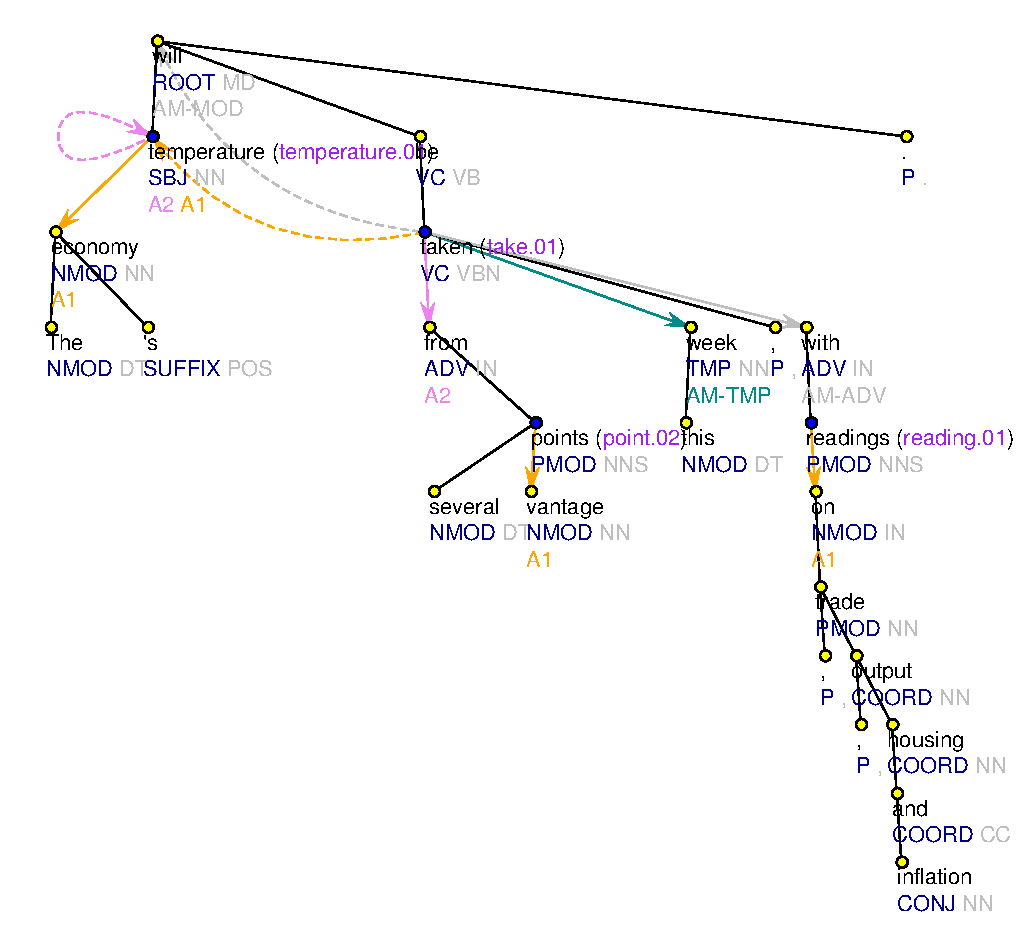
\includegraphics[height=4in,width=4.5in]{temperature-conll}
$\begin{array}{cc}
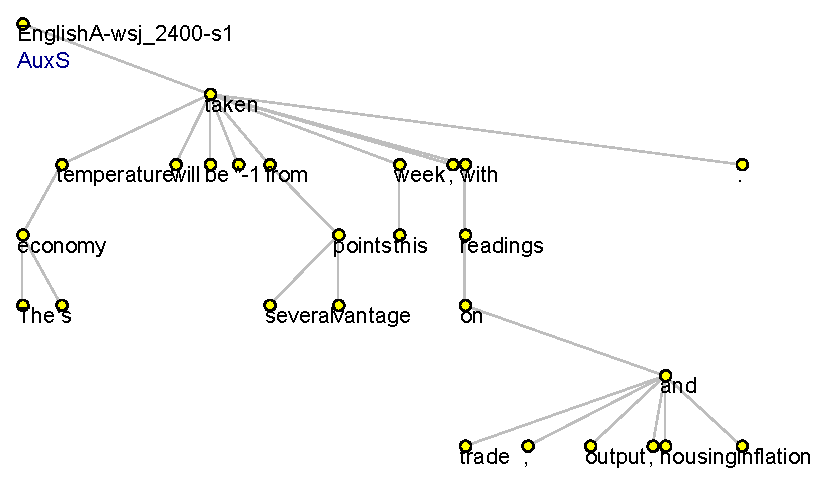
\includegraphics[height=2in,angle=270]{temperature-pedt-a} & 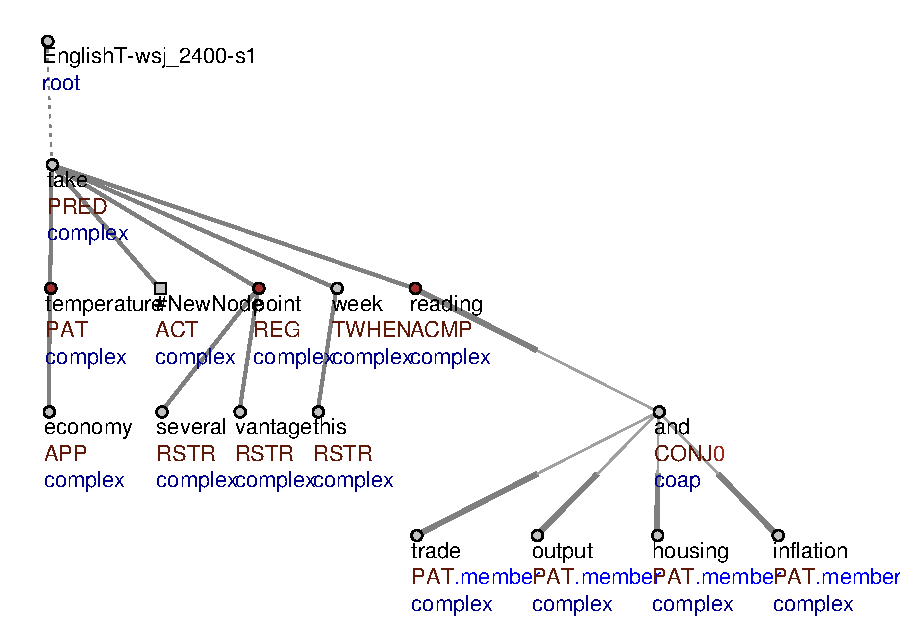
\includegraphics[height=2.75in,angle=270]{temperature-pedt-t}
\end{array}$
\end{center}
\end{figure}

A comparison of both annotations is shown in Figure \ref{fig:tree-comp}\footnote{The tree charts in this figure were created by the TrEd tree editor\\(\url{http://ufal.mff.cuni.cz/\~pajas/tred/}).}. It is apparent that the PEDT annotation encompasses richer semantic information, because it also contains semantic dependencies of adjectives and adverbs, as well as more detailed structure when compared to the two-level structure of PropBank and NomBank. The semantic role labels, which adhere to the FGD, are also different from the numbered arguments of PropBank and NomBank, even though the PEDT valency lexicon EngVALLEX \citep{semecky06} is originally based on PropBank and NomBank frames. While a wide labels remain semantically constant across different predicates, the most frequent valency arguments are subject to \emph{shifting} with verbs, i.e.\ the first argument of any verb is always called \texttt{ACT} and the second one \texttt{PAT}, even if they do not denote the semantic roles of an actor and an affected object, as it should be in a prototypical case\footnote{Cf. a detailed description in the annotation guidelines at: \\ \url{http://ufal.mff.cuni.cz/\~cinkova/TR\_En.pdf}, pg. 36ff. and 107ff.}. The references are treated in a different way as well: Additional links are inserted into the tree structure to represent them.

It is however still possible to find some common grounds between the two sources --- both of them include labeled dependencies between noun and verbal predicates and their required or voluntary arguments. The Czech part of the CoNLL 2009 contest included the PDT data whose annotation schema is also based on the FGD and uses the same dependency concept; therefore, it is probably feasible to adjust a SRL system designed for the CoNLL annotation for use with the PEDT data, as long as it remains within the limits of finding arguments of nominal and verbal predicates. Full semantic dependency parsing would probably require more radical modifications.

\section{The CoNLL Corpus: Data Format and Statistics}\label{data-format}

Since we have described the annotation schema and sources of the CoNLL 2009\footnote{As the concrete data format differs slightly from the 2008 version, we will now refer solely to the 2009 data sets used in this thesis.} corpus, we may now turn our attention to its technical implementation. The data is pre-divided into three sets: \emph{training}, \emph{development} (tuning) and (final) \emph{evaluation} sentences. Each of the sets is included in a single text file, which contains all the plain text, morphological, syntactic and semantic information. Each line in every text file comprises all the knowledge about one word (or punctuation sign), the individual types of inputs separated by tabs, forming columns. The purpose of each column is described in Table \ref{tab:st-columns}\footnote{Please see \url{http://ufal.mff.cuni.cz/conll2009-st/task-description.html} for additional explanation.}. Different sentences are divided by empty lines.

\begin{table}[htb]\footnotesize
\caption{The data columns of the CoNLL Shared Task corpus format}\label{tab:st-columns}
\begin{center}
\begin{tabular}{|r|l|l|}\hline
\bf No. & \bf Name & \bf Contents \\\hline
1 & ID & Number of the token in the sentence \\
2 & FORM & The word form as it appears in the original text \\
3 & LEMMA & Gold standard dictionary lemma of the word form \\
4 & PLEMMA & Automatically predicted lemma \\
5 & POS & Gold standard part-of-speech \\
6 & PPOS & Automatically predicted part-of-speech \\
7 & FEAT & \multirow{2}{*}{(Not used for English)} \\
8 & PFEAT & \\
9 & HEAD & ID of the syntactic head of this word (0 for root node; gold standard) \\
10 & PHEAD & Automatically predicted syntactic head ID \\
11 & DEPREL & Dependency relation label (gold standard) \\
12 & PDEPREL & Automatically predicted dependency relation label \\
13 & FILLPRED & Contains \texttt{Y}, if the word is a predicate \\
14 & PRED & The predicate name (lemma and sense number) \\
15+$i$ & APRED$i$ & Arguments of $i$-th predicate in the sentence \\\hline
\end{tabular}
\end{center}
\end{table}

\begin{figure}[p]
\caption{An example sentence from the CoNLL Shared Task Corpus}\label{fig:st-sample}
\begin{center}
\resizebox{\textwidth}{5cm}{
\begin{tabular}{llllllllllllllllllll}
1 & The & the & the & DT & DT & \_ & \_ & 2 & 2 & NMOD & NMOD & \_ & \_ & \_ & \_ & \_ & \_\\
2 & economy & economy & economy & NN & NN & \_ & \_ & 4 & 4 & NMOD & NMOD & \_ & \_ & A1 & \_ & \_ & \_\\
3 & 's & 's & 's & POS & POS & \_ & \_ & 2 & 2 & SUFFIX & SUFFIX & \_ & \_ & \_ & \_ & \_ & \_\\
4 & temperature & temperature & temperature & NN & NN & \_ & \_ & 5 & 5 & SBJ & SBJ & Y & temperature.01 & A2 & A1 & \_ & \_\\
5 & will & will & will & MD & MD & \_ & \_ & 0 & 0 & ROOT & ROOT & \_ & \_ & \_ & AM-MOD & \_ & \_\\
6 & be & be & be & VB & VB & \_ & \_ & 5 & 5 & VC & VC & \_ & \_ & \_ & \_ & \_ & \_\\
7 & taken & take & take & VBN & VBN & \_ & \_ & 6 & 6 & VC & VC & Y & take.01 & \_ & \_ & \_ & \_\\
8 & from & from & from & IN & IN & \_ & \_ & 7 & 7 & ADV & ADV & \_ & \_ & \_ & A2 & \_ & \_\\
9 & several & several & several & DT & DT & \_ & \_ & 11 & 11 & NMOD & NMOD & \_ & \_ & \_ & \_ & \_ & \_\\
10 & vantage & vantage & vantage & NN & NN & \_ & \_ & 11 & 11 & NMOD & NMOD & \_ & \_ & \_ & \_ & A1 & \_\\
11 & points & point & point & NNS & NNS & \_ & \_ & 8 & 8 & PMOD & PMOD & Y & point.02 & \_ & \_ & \_ & \_\\
12 & this & this & this & DT & DT & \_ & \_ & 13 & 13 & NMOD & NMOD & \_ & \_ & \_ & \_ & \_ & \_\\
13 & week & week & week & NN & NN & \_ & \_ & 7 & 7 & TMP & TMP & \_ & \_ & \_ & AM-TMP & \_ & \_\\
14 & , & , & , & , & , & \_ & \_ & 7 & 7 & P & P & \_ & \_ & \_ & \_ & \_ & \_\\
15 & with & with & with & IN & IN & \_ & \_ & 7 & 7 & ADV & ADV & \_ & \_ & \_ & AM-ADV & \_ & \_\\
16 & readings & reading & reading & NNS & NNS & \_ & \_ & 15 & 15 & PMOD & PMOD & Y & reading.01 & \_ & \_ & \_ & \_\\
17 & on & on & on & IN & IN & \_ & \_ & 16 & 16 & NMOD & NMOD & \_ & \_ & \_ & \_ & \_ & A1\\
18 & trade & trade & trade & NN & NN & \_ & \_ & 17 & 17 & PMOD & PMOD & \_ & \_ & \_ & \_ & \_ & \_\\
19 & , & , & , & , & , & \_ & \_ & 18 & 18 & P & P & \_ & \_ & \_ & \_ & \_ & \_\\
20 & output & output & output & NN & NN & \_ & \_ & 18 & 18 & COORD & COORD & \_ & \_ & \_ & \_ & \_ & \_\\
21 & , & , & , & , & , & \_ & \_ & 20 & 20 & P & P & \_ & \_ & \_ & \_ & \_ & \_\\
22 & housing & housing & housing & NN & NN & \_ & \_ & 20 & 20 & COORD & COORD & \_ & \_ & \_ & \_ & \_ & \_\\
23 & and & and & and & CC & CC & \_ & \_ & 22 & 22 & COORD & COORD & \_ & \_ & \_ & \_ & \_ & \_\\
24 & inflation & inflation & inflation & NN & NN & \_ & \_ & 23 & 23 & CONJ & CONJ & \_ & \_ & \_ & \_ & \_ & \_\\
25 & . & . & . & . & . & \_ & \_ & 5 & 5 & P & P & \_ & \_ & \_ & \_ & \_ & \_\\
\\
\end{tabular}
}
\end{center}
\end{figure}

\begin{table}[p]\footnotesize
\caption{Corpus size and coverage statistics for the CoNLL 2009 corpus used in this thesis}\label{tab:corpus-stats}
\begin{center}
\begin{tabular}{|c|rrrrrr|}\hline
  & \multirow{2}{*}{\bf Tokens} & \multirow{2}{*}{\bf Sentences} & \multicolumn{2}{c}{\bf Predicates} & \multicolumn{2}{c|}{\bf Coverage} \\
 & & & Distinct & All & Distinct & All \\\hline
Training & 958167 & 39279 & 9228 & 179014 & - & - \\
Development & 33368 & 1334 & 2151 & 6390 & 94.9~\% & 98.2~\% \\
Evaluation & 57676 & 2399 & 2610 & 10498 & 95.6~\% & 98.8~\% \\\hline
\end{tabular}
\end{center}
The figures shown are: the total number of tokens and sentences in the individual data sets, the number distinct predicates with the total number of predicate instances and for the development and evaluation data sets, the percentage of distinct predicates and their occurrences covered by the training set.
\end{table}

It is apparent from Figure \ref{fig:st-sample} that the corpus data format is very economic --- no data is repeated --- and easily human-readable. Manual analysis of corpus sentences is further simplified by the CoNLL 2009 Shared Task Extension for the TrEd tool\footnote{\url{http://ufal.mff.cuni.cz/\~pajas/tred/extensions/}}. On the other hand, the \texttt{APRED} columns and their different number for different sentences, as well as the fact that their order is only determined by the order of predicates in the sentence, clearly implies that such a data format is not well suitable as an input to the commonly used machine learning classifiers, since they require a constant data structure for the whole set, thus requiring a data conversion. This topic will be discussed further in Section \ref{conversion}.

The CoNLL corpus covers virtually all of the original PTB texts, while the vast majority of the data is designated for training purposes, as in most statistical learning problems. Table \ref{tab:corpus-stats} shows that most of the predicates and virtually all predicates with more than one occurrence in the development or evaluation set are covered by the training set, but a small group of unseen data will require to be treated separately.

The average number of predicates per sentence is $4.55$ in the training data set. Therefore, if the system is set-up to classify the arguments of one predicate at a time (which is the only straightforward option with classic machine learning approaches), the amount of data will multiply by that number. This results in effectively more training data instances and therefore possibly a higher classification precision. On the other hand, more computing resources will be needed to process such a large input.

%
%
\chapter{The Used Machine Learning Environment}\label{mlprocess}
%
%

In order to achieve an easy configurability of experiments needed for the SRL system setup and their fast parallel processing on multiple interconnected computers in a computing grid or cluster, we have designed and implemented a special software framework\footnote{Available online at \url{http://code.google.com/p/en-deep/} or on the enclosed CD, see Appendix \ref{cd-contents}.}. We have chosen the Java language for our program because of code portability, high performance and simple debugging and maintenance with the help of integrated development tools. We incorporated existing ML classifiers and other NLP tools into our system, as many of the freely available utilities feature a Java API\nomenclature{API}{Application Programming Interface}. We will now describe the basic concepts we applied in our implementation of the framework --- the decomposition of an experiment into subtasks (Section \ref{tasks}) and their batch processing (Section \ref{expansions}) in parallel (Section \ref{parallel}). We also attach an account of our integration of third-party libraries (Section \ref{weka}).

\section{Splitting the Experiments into Subtasks}\label{tasks}

As we described already in Section \ref{problem}, the whole SRL process that is the subject of this thesis consists of multiple subtasks. Having considered the pipeline approach to the system architecture and the implementation of multiple classifiers for different lemmas or senses (see Section \ref{related} for details), we realized that it will be profitable to divide the whole analysis into simple, compact subtasks and process some of them in parallel. It is apparent that for multiple classifiers or other operations on independent parts of the data, parallelization is a possibility which speeds up the whole process, thus allowing more time-consuming computation.

We have considered employing the GNU Make utility\footnote{\url{http://www.gnu.org/software/make/}}, but decided to create our own, more specific application, which would allow us to define our custom description of the task with simpler subtask specifications\footnote{This also includes the \emph{task expansions} described in Section \ref{expansions}.}, as well as launching the computation not only in multiple threads, but also in multiple processes running on different computers in a cluster.

We also decided to implement all the possible tasks as functions within a single executable application in order to reduce the OS overhead for process creation. The intended implementation in Java offered a simple concept which makes this possible while still maintaining modularity and extensibility: Every subtask is defined as a Java class derived from the base class called \texttt{Task}. In order to enable configurability, the individual settings or parameters of all the subtasks are then represented as name-value pairs handled by their concrete implementations\footnote{It is of course possible that some tasks do not need any parameters, which is regarded as an empty list of parameters. Similarly, binary parameters are viewed as parameters with an empty value.}. We divided all the tasks implemented in our system (See Appendix \ref{tasks-list} for a comprehensive list) into three groups for convenience: the classification, evaluation and data manipulation tasks.

Although many tasks may be processed in parallel without conflicts, there will necessarily be dependencies among some of them --- one subtask requiring the output of another subtask as it input. The dependencies should further be handled in such a way that it is still possible to use multiple machines in a cluster for the computation. We have chosen the only straightforward way to implement this, even if it poses a load on the interconnecting network: The inputs and outputs of all tasks are always saved to files. This further simplifies the description of the subtask dependencies --- it is possible to determine the necessary flow of the SRL process only by examining the names of input and output files of the individual tasks.

\begin{figure}
\caption{Subtask definition example}\label{fig:scenario}
\begin{center}
\begin{lstlisting}
# this is a commentary
task sttoarff; # id of the subtask
    algorithm: # used Java class
        en_deep.mlprocess.manipulation.StToArff;
    params: lang_conf="st-en.conf", # its settings
        divide_senses, one_file,  # parameters with no value (binary)
        generate="Children, DepPath, HeadPos", # parameters
        cluster_file="clusters-plain.txt";     # with values set
    in: "train.txt"; # inputs listing
    out: "train.arff"; # outputs listing
end;
\end{lstlisting}
\end{center}
\end{figure}

This all yields a task description which consists of a Java class name, its parameters and a list of inputs and outputs, which also define its dependencies and prerequisites. The whole experiment is then a list of such (sub)tasks. We represent the descriptions in a simple configuration file called the \emph{scenario} (see Figure \ref{fig:scenario}), which is parsed and topologically sorted \citep{kahn62} to create a to-do list or \emph{plan}, used by the individual running processes (see Section \ref{parallel}) to retrieve the next subtasks that need to be computed: Each subtask description in the plan contains an indication whether all of its prerequisites have already been completed.

\section{Wildcards and Task Expansion}\label{expansions}

Since we planned on using multiple machine learning classifiers or other operations which run multiple times on different data sets, we needed to have some means of describing that the same subtask should be launched in several variants. Therefore, we introduced simple wildcards into the description of the inputs and outputs of subtasks. An asterisk character (``*'') in a file name within the input or output specifications may stand for any string, thus forming a pattern. All the files from the current directory that match it are then transfered to the subtask definitions in the following two modes determined by the number of asterisks in the file name:
\begin{itemize}
    \item \emph{Expanding mode (``*'')}, which causes the subtask to \emph{expand} to multiple tasks, each taking one of the matching files. If there are multiple expanding mode patterns in the input specifications, only the corresponding ones, i.e.\ those where the ``*'' stands for the same string, are put together to create an expanded task (see Figure \ref{fig:expansion} for an example).
    \item \emph{Listing mode (``**'')}, which lets the subtask take all the matching files as its input, or create multiple matching files on the output. The output expansions are left up to the individual impelementations of the subtasks.
\end{itemize}

\begin{figure}
\caption{Task expansion example}\label{fig:expansion}\footnotesize
\begin{center}
Note that \texttt{data-a.dat} is not combined with \texttt{setting-b.dat}.

\begin{tabular}{m{3cm} c m{4.1cm} c m{4.1cm}}
\textbf{Work directory:}\par data-a.dat \par data-b.dat \par setting-a.conf \par setting-b.conf &
+ &
\textbf{Original Task:} \par \begin{lstlisting}
task sample;
# (...)
in: "data-*.dat",
    "setting-*.dat";\end{lstlisting} &
$\rightarrow$ &
\textbf{Expanded tasks:} \par \begin{lstlisting}
task sample^\#^a;
# (...)
in: "data-a.dat",
    "setting-a.dat";\end{lstlisting} \par \begin{lstlisting}
task sample^\#^b;
# (...)
in: "data-b.dat",
    "setting-b.dat";\end{lstlisting}
\end{tabular}
\end{center}
\end{figure}

These basic patterns were then further improved to suit all the batch processing needs during our experiments, so that they now allow for further specification enclosed in vertical bar (``\textbar'') characters immediately following the asterisk. The detailed specifications are ignored when determining the subtask dependencies, which allows to select inputs from different sources whose file names do not match (in contrast to the situation shown in Figure \ref{fig:expansion}), which results in a cartesian product. Further, it is possible to combine the two pattern modes, where at first, the listing mode is applied and then the expanding mode to the results of the first step.

The expansion of a task is also transferred to its dependencies, if they contain the expanding mode patterns in their input specifications. This is done already with the expansion of the prerequisite task, so that the individual computing processes (see Section \ref{parallel}) may start working on some of the expansions of the dependency even if other prerequisite expansions are not yet finished. However, the topological order of the whole plan is always preserved.

An important feature of our experiment framework is also the possibility that the individual tasks assign further subtasks themselves, which then occupy the immediately following position in the experiment plan. Inner dependencies of all such subtasks must then always result in one single termination subtask, so that the outer dependencies are left untouched. This allows for further parallelization of such time-consuming operations as greedy feature selection (see Section \ref{featsel}).

\section{Running the Tasks in Parallel}\label{parallel}

As we already mentioned in the previous sections of this chapter, our whole experiment software is designed to run in several instances in parallel. The number of working threads, i.e.\ the level of maximum possible parallelization along with the maximum possible load on the CPUs and data flow, is determined by the user: The main executable may be launched in multiple copies on the same machine, as well as on different computers in a networked cluster. There is also a possibility to start multiple threads within one program instance, which simplifies the usage with stand-alone multi-core machines.

The running threads are then completely independent of one another --- the only information exchange among them takes place in the plan file (see Section \ref{tasks}). Each thread will automatically parse the experiment scenario configuration file, if it does not find the plan file in the working directory, i.e.\ the first thread started will accept this duty. Consequently, all the working instances retrieve the pending subtasks from the plan file and remove the completed ones, while indicating that any depending subtasks are no longer blocked. The number of tasks retrieved at a time by one computing thread may be configured for the particular experiment based on the complexity of its subtask, so that program instances do not block each other and the input and output load on the plan file is not excessive.

If an error occurs within one of the subtasks, all the subtasks not depending on it will continue to be processed, so that the user can correct the error and relaunch only a part of the original plan. The logging feature with configurable verbosity and the possibility to launch a separate scenario parsing simplify the debugging of the experiment setup.

\section{Integration of Third-Party Libraries}\label{weka}

There is a wide variety of freely available NLP tools, such as classifiers or data filters, on the Internet. We decided to profit from some of them, while still keeping our experiment framework relatively independent. Therefore, the individual implementations of various subtasks in our system use the integrated tools, but the task descriptions, the scenario and plan file format and the mechanisms that launch them in the correct order are independent of any third-party tools\footnote{Google Collections (\url{http://code.google.com/p/google-collections/}) and Java-GetOpt (\url{http://www.urbanophile.com/\~arenn/hacking/getopt/}) are the only exceptions from this rule. They are invisible to the programmer who creates additional subtask algorithms, though.}. It is very simple to use additional Java libraries and programs with our system, since for each tool, only one wrapper Java class which defines the subtask and calls the particular tool with the correct parameters needs to be implemented.

We have chosen to integrate the Waikato Environment for Knowledge Analysis \citep[WEKA, ][]{garner95}\footnote{Version 3.7.1, \url{http://www.cs.waikato.ac.nz/~ml/weka/}}\nomenclature{WEKA}{Waikato Environment for Knowledge Analysis} with most of the subtasks our system, since it offers a very wide collection of ML classifiers, feature selection algorithms and data filters with a unified API and a transparent default data format --- the Attribute-Relation File Format (ARFF)\nomenclature{ARFF}{Attribute-Relation File Format}, which thus became the default format for our classification tasks.

As one of our classification subtasks makes use of the integer linear programming (ILP) technique (see \ref{post-inference}), we also included the LP\_Solve\footnote{Version 5.5, \url{http://lpsolve.sourceforge.net/}.} tool into our system. Although the program is written in the C++ programming language and called via a wrapper library using Java Native Interface (JNI)\nomenclature{JNI}{Java Native Interface}, which makes it less portable among different computer platforms, this problem is bound solely to the single subtask that uses this utility.

%
%
\chapter{Fundaments of Our Deep Analysis System}\label{ml-semantic}
%
%

We will now describe the basic strategy that we decided to pursue in the solution of our SRL problem (Section \ref{approach}), along with a brief explanation of the classification algorithms (from publicly available ML libraries) that we tested in our experiments (Section \ref{classifiers}). As we already mentioned in Section \ref{data-format}, the original data format of the used corpus is not well-suited for the operation of machine learning procedures. In addition, the set of properties for each word in the corpus does not describe the relations of the individual words. Therefore, we also include an account of our implementation of the data conversion (Section \ref{conversion}), as well as feature generation and selection (Sections \ref{features} and \ref{featsel}), all of which is required for proper classifier function and high performance output. Our system uses various generated features described by other authors and several additional, which we originally designed for the purpose of this thesis. The feature selection algorithms comprise our own application of well-known approaches, using ranking algorithms provided by the WEKA framework and our own implementation of the mRMR algorithm. We conclude this chapter with a description of the standard comparison metrics we adopted and programmed for our experiments (Section \ref{metrics}).

\section{Basic Approaches}\label{approach}

After careful consideration of the various machine learning solutions available (most of which were already discussed in Chapter \ref{related}), we decided to use the traditional supervised classifiers, such as SVM, MaxEnt or logistic regression, in our SRL system due to their competitive performance and simple configuration. The inclusion of many different algorithms in one software package, WEKA, and the extent of the available sources of information poses also an advantage of this choice.

It follows from the selected machine learning methods that it is now necessary to split the predicate disambiguation (PD) and argument classification (AC) task. The traditional classifiers are only able to infer the values of one target parameter at a time. Additionally, it is only needed to classify the predicates in the PD task, whereas all words could possibly appear as arguments of some of the predicates in the AC problem. The division among argument identification and argument labeling is then possible, but not necessary (please refer to Section \ref{ai-ac} for this particular topic).

The order in which these two subtasks will be processed is also not given. Although the reports of \citet{bohnet09} and \citet{zhao09} show that solving the AC problem before the PD problem may lead to very good results, after a preliminary analysis of the frame lexicons provided (see Section \ref{propbank-nombank}), we decided to take the more usual approach of disambiguating the predicates first, since the nature and number of arguments usually depends very closely on the predicate sense.

\section{Classifiers}\label{classifiers}

As we already pointed out in Chapters \ref{intro} and \ref{related}, the maximum entropy (MaxEnt) models \citep[p.~219ff.]{jelinek97} are one of the most used techniques in many different NLP tasks \citep[p.~607f.]{manning00} including SRL \citep{jiang06,zhao09,che09,chen09}. This is mainly thanks to the fact that their base idea of finding a conditional probability distribution with a maximum entropy \citep[average uncertainty][p.~61]{manning00} subject to given constraints, i.e.\ ``the most uniform model subject to our knowledge'' \citep[p.~41]{berger96} is very straightforward and effective. The basic form of the conditional probability model \citep{malouf02}, which predicts a probability of target event (such as semantic class) $y\in Y$ given a context $x$, looks as follows:
\begin{equation}
q_\theta(y|x) = \frac{\exp(\theta^T f(x,y))}{\sum_{y'\in Y} \exp(\theta^T f(x,y'))}
\end{equation}
The function $f$ represents an $N$-dimensional vector of features (see Section \ref{features}) and $\theta$ is the corresponding weight vector. The weights of the model are then trained to satisfy the maximum entropy condition, which is equivalent to minimizing the relative entropy \citep[or Kullback-Leibler Divergence;][p.~72]{manning00} of the model $q_\theta$ to the empirical distribution $p$ observed on the training data (expectation of the individual features' frequencies), or maximizing its a-posteriori probability (conditional probability given the training data), which is usually expressed in terms of the log-likelihood function:
\begin{align}\label{eq:maxent}
\begin{split}
\min_\theta D(p||q_\theta) & = \min_\theta \sum_{y,x} p(y,x) \log\frac{p(y|x)}{q_\theta(y|x)} \\
& = \max_\theta L(\theta) = \max_\theta \sum_{y,x} p(y,x) \log q_\theta(y|x) 
\end{split}
\end{align}
The techniques of fitting the model to the training data usually involve an iterative approach to the zero gradient of the log-likelihood function.

The \emph{logistic regression} \citep{hosmer00}, another very common classifier type, is a variant of a generalized linear regression model \citep{maccullagh91}. The following model form is used to predict the binary\footnote{It is, however, technically possible to classify multi-class target event using a binary classifier, e.g.\ by using multiple classifiers, each predicting one of the classes.} target event $y \in\{-1,1\}$ given a feature vector $x$ and a weight vector $\theta$ \citep{lee06}:
\begin{equation}
p(y|x,\theta) = \frac{1}{1 + \exp(-y\theta^T x)}
\end{equation}
The model is fitted to the training data $x_i,y_i;\ i = 1\dots p$ by maximizing its a-posteriori probability --- in a way analogous to MaxEnt (Equation \ref{eq:maxent}):
\begin{equation}\label{eq:logreg}
\max_\theta L(\theta) = \max_\theta \sum_{i=1}^p \log \frac{1}{1 + \exp(-y_i\theta^T x_i)} = \min_\theta \sum\log(1 + \exp(-y_i\theta^T x_i))
\end{equation}
This optimization problem is also solved using iterative methods \citep{fan08}. \citet{blower04} provides a proof that the logistic regression is equivalent to MaxEnt (for binary target events)\footnote{Cf.\ also the presentation by Pereira at:\\ \url{http://www.cis.upenn.edu/\~pereira/classes/CIS620/lectures/maxent.pdf}.}:
\begin{align}
\begin{split}
p(y=1|x) & = \frac{\exp(\theta^T f(x,1)}{\sum_{y'\in Y} \exp(\theta^T f(x,y'))} = \frac{\exp(\theta^T f(x,1))}{\exp(\theta^T f(x,1)) + \exp(\theta^T f(x,-1))} \\
& = \frac{1}{1 + \exp(-\theta^T f(x,-1))} = \frac{1}{1 + \exp(-\theta^T g(x))}
\end{split}
\end{align}
This gives us two variants of the same basic idea. Given that logistic regression is integrated into WEKA via the LibLINEAR\footnote{Version 1.51, \url{http://www.csie.ntu.edu.tw/\~cjlin/liblinear/}.} package \citep{fan08}, we decided to test the performance of this very classifier for our experiments.

Another widely used approach to classification is the \emph{support vector machine} \citep{boser92}. Its basic idea is representing the (training) data as points in $N+1$-dimensional space\footnote{This means that each feature, and also the target class corresponds to one dimension.}, whose coordinates are given by the function $\phi(x)$ of the features and by the value of the target event $y$, and trying to separate the different target events with a hyperplane that has the maximum margin (distance to the nearest point). If we assume that the target event $y$ is binary\footnote{Most SVM libraries are also capable of solving a problem with multiple target classes.} --- $y\in \{1,-1\}$, the hyperplanes that are parallel to the maximum margin separator and touch the nearest data points of both target classes (the \emph{support vectors}) are then described by the equations:
\begin{equation}
w^T x + b = 1\quad\mbox{and}\quad w^T x + b = -1
\end{equation}
Maximizing the distance $\frac{2}{||w||}$ leads to minimizing $||w||$ under the circumstances that the hyperplane fits the training data, which yields the following optimization problem \citep{hsu03}, given training examples $x_i,y_i;\ i = 1\dots p$:
\begin{equation}\label{eq:svm-primal}
\min_{w,b} \frac{1}{2}w^T w\quad\mbox{subject to}\quad y_i(w^T\phi(x_i) + b)\geq 1
\end{equation}
This may then be transformed using Lagrangian multipliers \citep{cristianini00}:
\begin{equation}
\min_{w,b} \max_{\alpha} \frac{1}{2}w^T w - \sum_{i=1}^p \alpha_i(y_i(w^T\phi(x_i) _ b) - 1)
\end{equation}
Now we may solve the equation using quadratic programming and get the solution $w = \sum_{i=1}^p \alpha_i y_i \phi(x_i)$, $\sum_{i=1}^p \alpha_i y_i = 0$, which finally results in the optimization problem:
\begin{equation}
\max_{\alpha} = \sum_{i=1}^p \alpha_i - \frac{1}{2}\sum_{i=1}^p y_i y_j \alpha_i \alpha_j (\phi(x_i)^T \phi(x_j))\quad\mbox{subject to}\quad \sum_{i=1}^p \alpha_i y_i = 0,\ \alpha_i = 0\ \forall i
\end{equation}
The $\phi(x_i)^T \phi(x_j)$ term is called the \emph{kernel} function, with the most usual kernels being linear\footnote{In the CoNLL 2009 contest, \citet{che09} describe using SVM with this type of kernel.} ($x_i^T x_j$) or radial ($\gamma x_i^T x_j + r)^d$). We chose to test some variants of SVMs in our experiments because of their reported high performance and usage simplicity: many different SVM types are integrated into WEKA through the LibLINEAR and LibSVM\footnote{Version 2.91, \url{http://www.csie.ntu.edu.tw/\~cjlin/libsvm/}.} \citep{chang01} libraries.

Since in most real-life classification problems, it is impossible to find a hyperplane that would separate both target event values for all training examples, a regularization \citep{neumaier98} term $\xi$ is introduced into the Equation \ref{eq:svm-primal}, which penalizes classification errors, transforming it to the following shape \citep{cortes95}:
\begin{equation}
\min_{w,b} \frac{1}{2}w^T w + C\sum_{i=1}^p \xi_i \quad\mbox{subject to}\quad y_i(w^T\phi(x_i) + b)\geq 1 - \xi_i
\end{equation}
The $C$ parameter is then interpreted as the penalty cost. There are several possible shapes of the regularization function for the SVM, most common being $L_1$ ($\max(1-y_i w^T x_i, 0)$) and $L_2$ ($\max(1-y_i w^T x_i, 0)^2$) norms, both of them integrated into LibLINEAR or LibSVM \citep{fan08,chang01}.

As correct classification of all the training examples may not be feasible with logistic regression, too, regularization is applied to it as well \citep{ng04,fan08}, which transfers the Equation \ref{eq:logreg} to the following form:
\begin{equation}
\min_\theta \sum\log(1 + \exp(-y_i\theta^T x_i)) + R(\theta)
\end{equation}
A function of the weight vector is used as the regularization term --- \citet{ng04} describe the application of $L_1$ and $L_2$ norms of $\theta$, the LibLINEAR version of logistic regression is $L_2$-regularized.

Since WEKA in the combination of LibLINEAR and LibSVM libraries provides the described high-performance classifiers out-of-the-box, we decided to apply them for our experiments. We also performed some simple preliminary tests with other traditional classifiers implemented in WEKA libraries, such as Decision Trees, Naive Bayes or Perceptron. However, their performance did not indicate that they could possibly surpass the selected ones by a significant margin and the need for other tests and (albeit minimal) reconfiguration would delay our work excessively.

\section{Data Conversion}\label{conversion}

In Section \ref{data-format}, we described the advantages and drawbacks of the input corpus data format. Since it is unsuitable for use with common ML classifiers, such as SVM or MaxEnt, in its original form, we needed to convert the sentences into the required layout with one instance, i.e.\ one token relating to one predicate, per line and a constant number of columns. We have designated the ARFF file format directly as the target of our conversion in order to easily use the generated files with WEKA classifiers (cf.\ Section \ref{weka}).

The conversion of each sentence looks as follows:
\begin{enumerate}
    \item The sentence is loaded and a unique ID is assigned to it, so that its data is easily recognized during the conversion process.
    \item For each predicate in the sentence, the following is done:
    \begin{enumerate}
        \item Each pre-selected word of the sentence (see below for data selection options) is taken and all the input CoNLL corpus columns (see Section \ref{data-format}), excluding all the \texttt{APRED} values, are augmented with more generated features, mainly regarding the context of the word with respect to the predicate (see Section \ref{features}) to generate one line of output.
        \item Only the value of \texttt{APRED} pertaining to the current predicate is added to the output line\footnote{At this point, it is also possible to separate the \texttt{APRED} values into two groups. For details, see Section \ref{arg-types}.}.
        \item The output lines for each pre-selected word in the sentence are written into the output file.
    \end{enumerate}
    This means that if there are e.g.\ five predicates in the sentence, it appears five times on the output, but always in relation to a different predicate.
\end{enumerate}

The precise character of the output file(s) and depends on the pre-set mode of operation. There are the following three settings regarding output file creation:
\begin{enumerate}
    \item An output file is created for each predicate lemma, i.e.\ all sentences with relation to the same predicate lemma are output into one file. The nominal and verbal predicates are also split, e.g.\ all sentences that contain the verbal predicate ``give'' fall into the file whose name contains ``give.v''. This serves the purpose of predicate disambiguation (see Chapter \ref{pd}).
    \item There is an output file for each predicate sense, e.g.\ ``give.01.v''. This is used for argument labelling (see Chapter \ref{ac}).
    \item All the data from one input file (e.g.\ the whole training set) are written into one output file. The predicates to which the data lines relate are indicated in a special column. This mode is also used in the argument labelling process.
\end{enumerate}

The selection of words that appear on the output may be set-up in the four following ways:
\begin{enumerate}
    \item Each word is selected, nothing is left out. This is used for the argument classification subtask.
    \item Only the predicates are selected. We use this setting for predicate disambiguation.
    \item A syntactic pruning algorithm \citep{asahara09,zhao09} is applied, so that only the ``syntactic neighborhood'' of the predicate is selected. We also tested this mode for predicate disambiguation (see section \ref{pruning}).
    \item Only tokens with the pre-selected part-of-speech values are selected. This is a somewhat simpler method of pruning, which has also been tested for predicate disambiguation (please refer to Section \ref{pruning} for details).
\end{enumerate}

This gives us a highly configurable tool that provides us with the input of all the various subtasks of our SRL solution.

\section{Generated Features}\label{features}

We will now turn our attention to the generated features already mentioned in Section \ref{conversion}. Since all the classifiers we used regard the training and testing instances (that is words that may belong to the same sentence) as independent, the input set of data columns (see Section \ref{data-format}) is insufficient as a feature set for the classification of one word, since it does not provide any information about other words in the sentence, which often co-determine its semantic characteristics. Therefore, additional features must be introduced that describe the particular word, its syntactical and topological neighborhood and the relations to other words in the sentence.

Our system is able to generate several types of features from the input data. To begin with, there are various qualities of the syntactical neighborhood of the given node and its relation to the predicate. The following types of features have been described by \citet{nugues09}, among others:
\begin{itemize}
    \item \emph{Siblings} --- word form, lemma, part-of-speech (POS)\nomenclature{POS}{Part-of-Speech} and \emph{coarse} POS (CPOS)\nomenclature{CPOS}{Coarse Part-of-Speech (first letter of the part-of-speech tag)} \citep[first character of the POS-tag;][]{che09} of the nearest syntactical siblings of the given word, if there are some.
    \item \emph{Dependency relation path} --- a string consisting of ``/'' (``up'') and ``\textbackslash'' (``down'') characters which describes the syntactic path from the given word to the predicate, interleaved with word forms, lemmas, POS, CPOS or the DEPREL labels (see Section \ref{data-format}) of the nodes encountered on the path, or left as such.
    \item \emph{Children} --- word forms, lemmas, POSs and CPOSs of the syntactic children of the given word.
\end{itemize}

There are further syntactic features, already reported by \citet{zeman09}, \citet{chen09} and \citet{asahara09}, and others:
\begin{itemize}
    \item \emph{Syntactic Dependence on Predicate} --- the value of this feature is ``1'', if the given word depends syntactically (even indirectly) on the predicate, ``0'' otherwise.
    \item \emph{Sibling or Child} --- ``1'', if the given word is a sibling or a direct child of the predicate, ``0'' otherwise.
    \item \emph{Head Position} --- the topological position relative to the syntactic head (Before, After).
    \item \emph{Head} --- word form, lemma, POS and CPOS of the syntactic head of the given word.
    \item \emph{Predicate} --- the same properties of the predicate; also in a bigram with the properties of the given word.
\end{itemize}

In addition to the listed syntactic features, we introduced the following feature type, which is, to our knowledge, new:
\begin{itemize}
    \item \emph{Children Types} --- this lists the word forms, lemmas, POSs and CPOSs and the total number of the children that belong to a word class. We distinguish the following word classes for the sake of this feature:
    \begin{itemize}
        \item Nominal POSs (nouns, adjectives and pronouns)
        \item Verbs (including modal verbs)
        \item Open POSs (nouns, adjectives, pronouns and verbs)
        \item Prepositions
        \item Particles
    \end{itemize}
\end{itemize}

We also include the following features that describe the topological neighborhood and morphological features of the given word:
\begin{itemize}
    \item \emph{Voice} --- the voice of the verb \citep{che09}, inferred from its POS and the POS of its head node.
    \item \emph{Left\dots Right} --- morphological features (form, lemma, POS, CPOS) of the first three words to the left and right of the given word, including a bigram for the first two in each direction.
    \item \emph{Position} --- the topological position relative to the predicate (Before, After, On) \citep{nugues09}.
    \item \emph{Word Distance} --- the topological distance from the predicate (absolute value, number of words separating the predicate and the given word) \citep{asahara09}.
\end{itemize}

The last type of features generated by our system, \emph{Cluster}, is our original concept, based on the technique of \emph{word clustering}\citep{pereira93}, which tries to select and group together words that usually appear in similar contexts, thus automatically creating classes of words that share similar semantic properties. We used the SenseClusters\footnote{Version 1.01, \url{http://senseclusters.sourceforge.net/}.} tool \citep{kulkarni05} to generate clusters on word forms and lemmas as they appear in the original corpus sentences, also in combination with POS, thus creating a group of features that involve the different cluster types for topological and syntactical neighbors\footnote{In particular, they are analogous to the Left\dots Right, Dependency path, Head, Siblings and Children features.} of the given word.

\section{Feature Filtering and Selection}\label{featsel}

Given such a large set of features as described in Section \ref{features} (consisting of up to 150 features), it is very probable that some of them will be irrelevant or redundant for the inference of the target class \citep{john94}, or even introduce noise that increases the classification error \citep[p.~251]{manning08}. Therefore, we needed to implement some feature filtering and selection techniques.

As to the feature filtering, we implemented and apply these two simple techniques in our system:
\begin{enumerate}
    \item \emph{Filtering irrelevant attribute values} --- for most features with multiple string values, such as Children, Dependency path or Left\dots Right, we filter all the values that do not occur very often in the training data and unify them under a new single value, ``other''. This removes all values that would otherwise be ignored by the classifier or introduce noise. This is analogous to frequency-based selection described by \citet[p.~257]{manning08}.
    \item \emph{Filtering irrelevant attributes} --- we filter all the attributes that are, in the given case, obviously irrelevant, i.e.\ they either do not contain any value which would repeat in the training data, or are constant across the whole training set.
\end{enumerate}

In addition to filtering, one must select a subset of features that yields the optimal performance. For this purpose, the usual approach is to train the classifier iteratively for different feature subset and evaluate its performance on the \emph{development} data set (see Section \ref{data-format}), thus obtaining the best performing subset. Since it is not computationally feasible to try every possible combination of features, we have to apply faster algorithms that may produce a suboptimal solution. We employ our own implementation of two different basic techniques in our SRL setup, applying parallelization:
\begin{enumerate}
    \item \emph{Feature ranking} --- the features are ordered according to a given criterion (see below) and the $N$ best are selected \citep[p.~251ff.]{manning08}. In our system, we usually gradually increase the $N$ in a certain range and then select the best value. All trials for different $N$ may be launched in parallel.
    \item \emph{Greedy algorithm} --- this iterative algorithm keeps a set of features and tries to add all the remaining features in each step, then selects the best one \citep{caruana94}. In our setting, we either start with one feature, or try all possible combinations in a small subset of features (with the best ranking). Of equally performing features, we always select the one that has been rated as the best one in the ranking. Each round trying to add all remaining features may be processed in parallel.
\end{enumerate}

Our system contains the following feature ranking criteria:
\begin{itemize}
    \item \emph{$\chi^2$-Criterion} \citep[p.~255]{manning08} --- this evaluates the features using the $\chi^2$-statistics against the target feature, which is computed as $\sum_{f\in F}\sum_{t\in T}\frac{(N_{ft}-E_{ft})^2}{E_{ft}}$, where $f,t$ are all possible values of the feature $F$ and the target $T$, respectively, and $E,N$ are the expected and observed frequencies of the values occurring together.
    \item \emph{Mutual Information} (MI)\nomenclature{MI}{Mutual Information} \citep[p.~583]{manning00}, or \emph{Information Gain} \citep[p.~264]{manning08} --- this computes the difference of the entropy of the target feature alone and the conditional entropy of the target feature given the ranked feature, that is how much the knowledge of this feature lower the entropy of the target one.
    \item \emph{Symmetric Uncertainty} \citep[p.~291f.]{witten05} --- this statistics is defined as $\frac{2I(F,T)}{H(F) + H(T)}$, where $H$ is the entropy, $I$ is the MI and $F,T$ stand for the evaluated and target feature, respectively.
    \item \emph{ReliefF} \citep{kira92,kononenko94} --- this is an algorithm that ranks the features depending on how well they distinguish between the values of the target event: In a pre-set number of iterations, it selects random instances and then searches for the ``nearest hit'' (nearest instance, based on the value of the ranked feature, that has the same target event class) and ``nearest misses'' with different classes. The worth of the feature is then a sum of distance differences between the hits and misses weighted by the probability of possible target feature values.
    \item \emph{Significance} \citep{ahmad05} --- this algorithm is based on a similar assumption to the previous one, namely that a ``valuable'' feature should differentiate between the values of the target event. Given the training data statistics, it computes the average probability of the most probable set of target classes (the ``support set'') for each value  of the evaluated feature, then a symmetric value describing the most probable sets of the evaluated feature values for each target class. The average of the two values is then returned as the final rank.
    \item \emph{Minimum Redundancy-Maximum Relevance} (mRMR)\nomenclature{mRMR}{Minimum Redundancy-Maximum Relevance} \citep{peng05} --- using the concept of MI, this technique maintains a set of features, starting with an empty set, and greedily selects a feature that is most relevant to the target event, but not too redundant with respect to the already selected features. This feature is a solution to the following optimization problem (where $S_{m-1}$ is the currently selected set of features):
\begin{equation}
\max_{F_j\not\in S_{m-1}} \left[ I(F_j,T) - \frac{1}{m-1} \sum_{F_i\in S_{m-1}} I(F_i,F_j)\right]
\end{equation}
\end{itemize}
All the criteria but mRMR were integrated into the WEKA framework; we implemented the mRMR ranking algorithm (including our own implementational variant of MI, which we also use in the rankings) for the purpose of this work. We also made performed tests with averaging the rankings --- either all the rankings or only mRMR and ReliefF, following the ideas of \citet{zhang08} in a simplified way, so that the average is less prone to possible failures of one of the ranking algorithms.

Our decision to apply or combine the various rankings or to employ the greedy algorithm in the individual subtasks in our system (see Chapters \ref{pd} and \ref{ac}) depends on the complexity and data volume in the particular case and is a trade-off between computation speed and final classifier performance.

Moreover, we always convert the multiple-valued string features to a set of binary features, each indicating the presence of one possible value, as the classifiers used in our experiments interpret all features as numeric\footnote{We chose to perform the binarization only after feature selection, since this reduces the computation time needed. Selecting the binarized features would probably improve the performance, but also retard the process on the other hand.}. The values of numeric attributes are then normalized \citep[p.~56f.]{witten05} to lie within the $[0,1]$ interval, so that the classifiers may use them as a metric.

\section{Measuring the Classifier Performance}\label{metrics}

In order to compare the different subtask configurations of our system, we adopted the standard metrics used in NLP tasks \citep[p.~268ff., p.~142ff., p.~171ff., respectively]{manning00,manning08,witten05} --- \emph{accuracy}, \emph{precision and recall}  and \emph{$F$-measure} ($F_1$)\footnote{We implemented a simple evaluation subtask that is able to compute all four of them.}.

Accuracy is the most straightforward one of them; it is computed as the percentage of correctly classified (\emph{true}) data instances.
\begin{equation}
A = \frac{t}{t + f}
\end{equation}
In the equation, $t$ stands for true examples and $f$ for \emph{false} (wrongly classified) instances. It is obvious that this measure can be used for multi-class problems, such as the PD problem (see Chapter \ref{pd} for its application in our system).

The other measures of comparison are based on the concept of \emph{negative} and \emph{positive} data instances. It relates to a binary classification problem situation where a part of the data is relevant and needs to be retrieved. Such data examples are called positive, whereas the rest of the input is referred to as negative. Precision and recall lay a greater focus on the positive examples, since their number is usually much smaller than that of the negative ones, which could lead to all instances being classified as negative if the ultimate goal was to maximize accuracy.

The formulas for computing precision and recall are defined in the following way ($tp,tn$ being true positive and negative instances and $fp,fn$ false positive and negative instances, respectively):
\begin{equation}
P = \frac{tp}{tp + fp},\quad R = \frac{tp}{tp + fn}
\end{equation}
Maximizing precision thus means improving the system, so that it does not retrieve irrelevant data, while maximizing recall means striving to retrieve as much relevant data as possible, regardless of false positives. In many situations including SRL, it is important for the optimum performance of a solution that both precision and recall stay high. Therefore, an additional metrics has been introduced, which makes a compromise between them --- the $F$-measure. The most usual variant, $F_1$, which weighs precision and recall equally, computes as the harmonic mean of the two values:
\begin{equation}
F_1 = \frac{1}{\frac{1}{P} + \frac{1}{R}} = \frac{2PR}{P+R}
\end{equation}

In the CoNLL 2009 contest, a \emph{labeled} variant of precision, recall and $F_1$ \citep{hajic09} was used in addition to the standard versions to compare the results of the competing SRL systems. It uses the same notion of positive and negative examples, while effectively counting correctly retrieved, but wrongly labeled data instances as both false positive and false negative. We adopted this approach for our AC system (see Chapter \ref{ac}), since it both measures the correctness of the semantic labeling and focuses on the positive instances, i.e.\ semantic arguments.

For the total evaluation of the whole system, we used the original CoNLL 2009 scorer\footnote{\url{http://ufal.mff.cuni.cz/conll2009-st/scorer.html}}, which computes labeled and unlabeled precision, recall and $F_1$ scores, while combining predicate senses with semantic arguments.

We also needed to measure the relevance of a performance difference between two variants of a subtask configuration in terms of one of the above metrics. For this purpose, we adopted and implemented the \emph{bootstrap} technique \citep[p.~152]{efron79,witten05}, which is very fast to compute and renders reliable results. We chose not to use other commonly applied approach, the \emph{cross-validation} \citep[p.~241ff.]{hastie09}, due to its higher computational requirements.
The bootstrap is calculated in the following way: By iteratively selecting random subsets of the original output and determining the classifier performance on these subsets, we obtain an estimate of the probability distribution for the classifier output, whose percentiles give the desired confidence interval (90~\% is used in this thesis). In conclusion, if the confidence intervals for two classifier variants do not overlap, one of them performs significantly better.

%
%
\chapter{Predicate Disambiguation}\label{pd}
%
%

This chapter contains the technical description of our own implementation of the predicate disambiguation, the first part of our SRL system. We have split the PD problem into several parts, according to the nature of the particular predicates (see Chapter \ref{pd-observe}), and applied various ML techniques described in Chapter \ref{ml-semantic}. An account of our approach to classifier parameter tuning (using the third-party classifier libraries selected in Section \ref{classifiers}) is given in Section \ref{classifier-setting}, followed by the feature selection techniques (employing our own implementations of well-known algorithms, together with library-supplied feature rankings) in Section \ref{pd-training}. We will then include an overview of the whole PD solution (Section \ref{pd-overview}).

\section{Observations on the Data}\label{pd-observe}

The first and most significant observation we made on the data is that as all predicate labels consist of a lemma and a sense number, it is evident that predicate senses for different lemmas are completely independent of each other. Further, since the numberings for nouns and verbs overlap, nominal and verbal predicates must be treated as separate problems. This implies that splitting the data according to the lemma and training a separate classifier for each lemma is profitable, since this prevents the machine learning algorithm from selecting an incorrect lemma at all times, even with rare predicates. We therefore adopted this practice, similarly to \citet{che09} and \citet{nugues09}. Our data-conversion algorithm (introduced in Section \ref{conversion}) thus produced only the predicate words as the input for the entire PD task, split into individual files according to the predicate lemma\footnote{We will henceforth consider predicate lemmas to be distinct for nouns and verbs, which is technically insured by the conversion process, appending the POS indication after the predicate lemma (e.g.\ ``progress.v'').}.

As we already mentioned in Section \ref{data-format} and depicted in Table \ref{tab:corpus-stats}, a very broad range of predicates occurs in the CoNLL 2009 corpus, with a small subset of them appearing only in one or two of the data sets. Additionally, Table \ref{tab:lemma-stats} shows the numbers of predicate lemmas and their coverage. We must therefore distinguish among the following cases:
\begin{enumerate}
    \item There are training and development instances of the given predicate lemma. \\
This is by far the most common case, not only regarding the number of the unique lemmas, but mainly with respect to the number of instances. We are able to tune the classifier setting on the development set for such predicates.
    \item Only training instances are available. \\
In that case it is possible to train the classifier, but no tuning can be done.
    \item There are no training data for the particular predicate lemma. \\
With no training data, only a dummy classifier that assigns always the same value is possible.
\end{enumerate}
This division does not take the evaluation data into consideration, apart from the fact that it is ready for previously unseen predicates. We can solve the individual cases and prepare the best possible classifier setting, which is then used only for those predicates that actually occur in the evaluation data.

\begin{table}[htbp]\footnotesize
\caption{Predicate lemma statistics for the CoNLL 2009 corpus}\label{tab:lemma-stats}
\begin{center}
\begin{tabular}{|c|rrr|}\hline
& \bf Predicates  &\bf Lemmas & \bf Coverage (Lemmas) \\\hline
Training & 9228 & 7639 &  - \\
Development & 2151 & 1946 & 95.5~\% \\
Evaluation &  2610 & 2337 & 96.2~\%  \\\hline
\end{tabular}
\end{center}
The values shown are the total numbers of distinct predicates and distinct predicate lemmas, followed by the percentage of predicate lemmas in the development and evaluation sets covered by the training set.
\end{table}

There is another distinction that must be done prior to the actual classifier training, namely based on the number of senses for each predicate lemma. As is evident from Table \ref{tab:senses-num}, a vast majority of the lemmas has a unique sense (we will refer to them as \emph{unary}). In total, a larger part of all predicate occurrences, although not as predominant, falls within this group. This renders the classification of those lemmas trivial; we will therefore always assign the only observed sense to them.

\begin{table}[htb]
\caption{Number of senses for the individual predicate lemmas as observed in the training data set}\label{tab:senses-num}\footnotesize
\begin{center}
\begin{tabular}{|r|rrr|rrr|}\hline
\multirow{2}{*}{\bf Senses} & \multicolumn{3}{c|}{\bf Predicate Lemmas} & \multicolumn{3}{c|}{\bf Number of occurrences} \\
 & Total & \% & Group & Total & \% & Group \\\hline
1 & 6541 & 85.6 & 6541 & 112994 & 63.1 & 112994 \\\hline
2 & 773 & 10.1  & \multirow{2}{*}{961} & 27395 & 15.3 & \multirow{2}{*}{41801} \\
3 & 188 & 2.4 & & 14406 & 8.0 & \\\hline
4 & 66 & 0.8 & \multirow{4}{*}{120} & 7726 & 4.3 & \multirow{4}{*}{16291} \\
5 & 24 & 0.3 & & 3571 & 2.0 & \\
6 & 13 & 0.2 & & 1745 & 1.0 & \\
7 & 13 & 0.2 & & 2522 & 1.4 & \\
8 & 4 & 0.0 & & 727 & 0.4 & \\\hline
9 & 3 & 0.0 & \multirow{11}{*}{17} & 883 & 0.5 & \multirow{11}{*}{7928} \\
10 & 3 & 0.0 & & 929 & 0.5 & \\
11 & 3 & 0.0 & & 882 & 0.5 & \\
12 & 2 & 0.0 & & 1638 & 0.9 & \\
13 & 1 & 0.0 & & 141 & 0.0 & \\
14 & 2 & 0.0 & & 1105 & 0.6 & \\
15 & - & - & & - & - & \\
16 & - & - & & - & - & \\
17 & 1 & 0.0 & & 585 & 0.3 & \\
18 & 1 & 0.0 & & 809 & 0.5 & \\
19 & - & - & & - & - & \\
20 & 1 & 0.0 & & 956 & 0.5 & \\\hline
\end{tabular}
\end{center}
The Group column contains the total numbers of lemmas assigned to the individual groups (unary, simple, harder, tough).
\end{table}

However, still a large number of predicate lemmas are not unary. We have divided them into three groups, which we treat differently. Most lemmas sport only two or three senses; we denote such lemmas \emph{simple}, for their classification problems are not very complicated (as the number of instances is also not very high on average). This makes the classifier tuning less important and shifts the stress on the speed of the solution, so that all of the lemmas can be processed within a reasonable amount of time.

Another, smaller group of predicate lemmas subsumes a greater number of senses (four to eight, labeled \emph{harder}). There are still considerably many such lemmas --- therefore, the adjustment of the classifier must be more sophisticated, but still fast enough, so that our system can cope with many lemmas of this kind.

The last, but important group of lemmas is highly ambiguous (we will refer to them as \emph{tough}) --- in most cases it is functional verbs and verbs that serve as the base element of multiple phrasal verbs, such as ``go'', ``take'', ``get'' etc. Only very few nominal lemmas belong to this group, all of them representing very abstract and vague terms --- ``line'', ``way'', ``place'', ``hand''. We believe that for such a small subset, a more time-consuming, but very accurate tuning algorithm should be applied.

\section{Selecting the Classifier Setting}\label{classifier-setting}

We have decided to use the same ML classifier with a constant set of parameters for the whole task, because selecting the best algorithm and configuration for each predicate lemma would complicate the training process and increase its duration excessively. Therefore, we needed to obtain a classifier and a set of parameters with the highest performance in an average case. We thus created an experiment that would test several classifier types from the LibLINEAR and LibSVM packages (as indicated in Section \ref{classifiers}) with many different settings and compare them to each other. We used \emph{accuracy} as the measure of comparison for the individual configurations, since the PD task is a multi-class problem with no well-defined ``positive'' and ``negative'' data instances, which are needed for all other standard metrics described in Section \ref{metrics}.

Since the size of the input corpus is too great to test each pre-selected algorithm and configuration on the whole development set, we created a smaller subset of both training and development data for our experiments (referred to as \emph{PD Experimental Subset}), selecting 100 predicate lemmas with the biggest development data sets. Since most of the plentifully represented predicates are also more ambiguous than the average, such a selection shows convenient for finding a configuration that would suit best to the harder and tough lemmas, where the parameter tuning is of highest importance.

We planned to apply feature selection to the training algorithms and hence took it into account for this experiment as well\footnote{Feature filtering and selection preliminaries are described in detail at the beginning of Section \ref{pd-training}.}: Our system used the filtering and all the feature rankings discussed in Section \ref{featsel} and tried to find the optimal number of features in the range\footnote{If less features remain after the filtering, all of them are examined in the same fashion. This also applies to the following feature selection variants.} $4-30$ by consecutively trying to add the next one in the order given by the particular ranking, then selected the best result of the individual rankings\footnote{We apply the same feature selection technique to harder lemmas in our PD system. Cf. Section \ref{pd-training} for details.}. We then averaged the results of each classifier setting for all the lemmas in our subset and established an estimate of confidence intervals using the bootstrap method (see Section \ref{metrics}).

\begin{table}[htbp]
\caption{Classifier performance on the PD Experimental Subset with feature ranking}\label{tab:pd-classifiers}\footnotesize
\begin{center}
\shorthandoff{-}
\begin{tabular}{|l|l|l|c|c|c|}\hline
\bf Software & \bf Classifier & \bf Parameters & \bf Acc. & \bf 5~\% & \bf 95~\% \\\hline
\multirow{24}{*}{LibLINEAR} & \multirow{4}{*}{$L_2$-Log. Regression} & C = 2; E = 0.001 & \bf 92.9 & 91.3 & 94.5 \\
 & & C = 5, 10; E = 0.001 & 92.8 & 91.1 & 94.5 \\
 & & C = 1; E = 0.001 & 92.7 & 91.0 & 94.4 \\
 & & C = 5; E = 0.01 & 92.7 & 91.0 & 94.4 \\\cline{2-6}
 & \multirow{5}{*}{Multiclass SVM} & C = 2; E = 0.001, 0.01, 0.1 & \bf 92.9 & 91.3 & 94.5 \\
 &  & C = 0.05; E = 1 & 92.8 & 91.0 & 94.4 \\
 &  & C = 0.1; E = 0.001, 1 & 92.8 & 91.2 & 94.2 \\
 &  & C = 2; E = 1 & 92.8 & 91.3 & 94.4 \\
 & & C = 5; E = * & 92.8 & 91.1 & 94.6 \\\cline{2-6}
 & \multirow{5}{*}{$L_1$-SVM (Dual)} & C = 2; E = 0.001, 0.01, 0.1 & \bf 92.9 & 91.2 & 94.4 \\
 & & C = 0.05; E = 1 & 92.8 & 91.2 & 94.4 \\
 &  & C = 0.1; E = 0.001, 1 & 92.8 & 91.1 & 94.4 \\
 & & C = 2; E = 1 & 92.8 & 91.1 & 94.5 \\
 & & C = 5; E = * & 92.8 & 91.1 & 94.4 \\\cline{2-6}
 & \multirow{5}{*}{$L_2$-SVM (Dual)} & C = 2; E = 0.001, 0.01, 0.1 & \bf 92.9 & 91.1 & 94.4 \\
 &  & C = 0.05; E = 1 & 92.8 & 91.2 & 94.4 \\
 &  & C = 0.1; E = 0.001, 1 & 92.8 & 91.2 & 94.5 \\
 &  & C = 2; E = 1 & 92.8 & 91.1 & 94.4 \\
 & & C = 5; E = * & 92.8 & 91.1 & 94.5 \\\cline{2-6}
 & \multirow{5}{*}{$L_2$-SVM (Primal)} & C = 2; E = 0.001, 0.01, 0.1 & \bf 92.9 & 91.1 & 94.5 \\
 &  & C = 0.05; E = 1 & 92.8 & 91.2 & 94.4 \\
 &  & C = 0.1; E = 0.001, 1 & 92.8 & 91.2 & 94.4 \\
 &  & C = 2; E = 1 & 92.8 & 91.2 & 94.5 \\
 &  & C = 5; E = * & 92.8 & 91.1 & 94.4 \\\hline
 \multirow{4}{*}{LibSVM} & \multirow{2}{*}{Linear Kernel} & C = 2, 5 & \bf 93.1 & 91.4 & 94.6 \\
 &  & C = 1, 10 & 92.8 & 91.2 & 94.5 \\\cline{2-6}
 & \multirow{2}{*}{Radial Kernel} & C = 2, 5; $\gamma$ = * & \bf 93.1 & 91.5 & 94.6 \\
 &  & C = 1, 10; $\gamma$ = * & 92.8 & 91.1 & 94.4 \\\hline
\end{tabular}
\shorthandon{-}
\end{center}
The listed values are: accuracy percentage on the whole experiment set, bootstrap 5~\%-percentile and bootstrap 95~\%-percentile. Only up to five best performing configurations for each classifier are listed; if the performance on the whole set is identical, the figures are merged and only the outermost bootstrap values are shown. An asterisk (``*'') in the parameters specifications signifies that any of the tested values is possible.
\end{table}

We discovered in our preliminary experiments with no feature selection that if the regularization penalty cost parameter is set higher than $10$, the performance of all classifiers is lowered and training duration becomes much longer. Additionally, lower termination criterion for the iterative fitting step of LibLINEAR classifiers than $0.001$ does not change the algorithm output. We have therefore pre-selected the parameter values accordingly and examined the following classifier setups:
\begin{itemize}
    \item $L_2$-regularized logistic regression from the LibLINEAR package, with the penalty cost parameter $C\in\{0.05,0.1,0.2,0.5,1,2,5,10\}$ and the termination criterion $E=\{0.001, 0.01, 0.1, 1\}$.
    \item $L_2$-SVM primal and dual problem, $L_1$-SVM dual problem and multi-class SVM from the LibLINEAR package, with the same penalty cost and termination criterion parameters as previous.
    \item C-SVM with a linear kernel from the LibSVM package, with the penalty cost parameter $C\in\{0.05,0.1,0.2,0.5,1,2,5,10\}$.
    \item C-SVM with a radial basis kernel from the LibSVM package, with the same regularization cost and the parameter $\gamma\in\{0.001,0.01,0.1,1\}$.
\end{itemize}
The list of the best-performing classifier algorithms and parameter settings, along with their results, is given in Table \ref{tab:pd-classifiers}. It is now apparent that the various classifiers perform very similarly; the results of the individual SVM variants from the LibLINEAR package are almost identical. The confidence intervals estimated by bootstrap overlap for all the algorithms, and thus higher accuracy on the experiment data set cannot be considered a decisive criterion for selecting one of them.

However, the results of the test also show that all of the classifiers are relatively sensitive to parameter settings. The logistic regression stays under 87~\% accuracy with the termination criterion set at $1$, independent of the cost value; however, its results remained at the top level as long as this this variable was set at $0.01$ or lower. Both LibSVM classifiers reach only approximately 90~\% accuracy with inadequate configuration. The LibLINEAR SVM methods are less prone to misconfiguration, their worst outputs rate at 91.8~\%. It is also apparent from Table \ref{tab:pd-classifiers} that the regularization penalty $C$ set at $2$ proves to be optimal for all the machine learning techniques, albeit by a very narrow margin.

\begin{table}[htpb]
\caption{Classifier performance on the PD Experimental Subset with no feature selection}\label{tab:pd-allfeat}\footnotesize
\begin{center}
\shorthandoff{-}
\begin{tabular}{|l|l|l|c|c|c|}\hline
\bf Software & \bf Classifier & \bf Parameters & \bf Acc. & \bf 5~\% & \bf 95~\% \\\hline
\multirow{11}{*}{LibLINEAR} & \multirow{3}{*}{$L_2$-Log. Regression} & C = 0.1; E = 0.1 & \bf 91.5 & 89.5 & 93.1 \\
 & & C = 0.1, 0.5; E = 0.001 & 91.4 & 89.7 & 93.1 \\
 & & C = 0.1; E = 0.01 & 91.4 & 89.7 & 93.1 \\\cline{2-6}
 & \multirow{2}{*}{Multiclass SVM} & C = 0.05; E = 0.1, 0.01, 0.001 & \bf 91.1 & 89.3 & 92.8 \\
 &  & C = 0.1; E = 0.01 & 90.6 & 88.9 & 92.4 \\\cline{2-6}
 & \multirow{2}{*}{$L_1$-SVM (Dual)} & C = 0.05; E = 1 & \bf 91.5 & 89.8 & 93.3 \\
 & & C = 0.05; E = 0.001 & 91.4 & 89.5 & 93.2 \\ \cline{2-6}
 & \multirow{2}{*}{$L_2$-SVM (Dual)} & C = 0.05; E = 1 & \bf 91.2 & 89.4 & 93.0 \\
 &  & C = 0.05; E = 0.1,0.01,0.001 & 91.1 & 89.3 & 92.8 \\\cline{2-6}
 & \multirow{2}{*}{$L_2$-SVM (Primal)} & C = 0.05; E = 0.001 & \bf 91.4 & 89.5 & 93.1 \\
 &  & C = 0.05; E = 0.01 & 91.2 & 89.4 & 92.8  \\\hline
 \multirow{4}{*}{LibSVM} & \multirow{2}{*}{Linear Kernel} & C = 0.1, 0.2 & \bf 86.7 & 84.5 & 88.9  \\
 &  & C = 1, 2 & 86.3 & 84.2 & 88.4 \\\cline{2-6}
 & \multirow{2}{*}{Radial Kernel} & C = 2; $\gamma$ = 0.001 & \bf 89.1 & 87.2 & 91.1 \\
 &  & C = 5, 10; $\gamma$ = 0.001 & 88.9 & 86.9 & 90.8 \\\hline
\end{tabular}
\shorthandon{-}
\end{center}
The format of this table is the same as in Table \ref{tab:pd-classifiers}. Only a maximum of three best settings is listed.
\end{table}

In order to test classifier sensitivity to irrelevant features, we performed a variant of the above experiment with the same software and configuration, but no feature selection, i.e.\ all the filtered generated features were present in the classifier inputs. Table \ref{tab:pd-allfeat} lists the results of this trial, which showed that the performance of the LibSVM classifiers depends very strongly on the relevance of the input features. All the LibLINEAR methods proved superior, with the results of logistic regression performing slightly better than the SVM algorithms. In addition, the results of all LibLINEAR models and the LibSVM linear kernel SVM for different parameters do not vary nearly as much as with feature selection (the highest interval between the best and the worst result was 1.1~\% with $L_1$-SVM). The LibSVM radial kernel SVM is very sensitive to the parameter values --- their proper setting yields as much as $5$ accuracy percent points difference.

As a result of this experiment, we have chosen to perform the PD task classification with the $L_2$-regularized logistic regression from the LibLINEAR package, for it reaches very high performance with most configurations, provided the termination criterion parameter is low enough. Therefore, this variable was set at $0.001$ for all subtasks, and the penalty cost remained at $2$.

\section{Feature Selection Approaches}\label{pd-training}

Having selected the classifier settings, we focused on perfecting the feature selection techniques for the individual groups of predicate lemmas identified in Section \ref{pd-observe}. In our preliminary experiments on small data sets, we found it profitable to filter out all feature values that occur in less than 1~\% of training instances and less than three times, we therefore use the filtering methods as described in Section \ref{featsel} in this particular configuration. We also learned that using more than about 30 features is not likely to improve the classifier performance, as for every individual lemma, many features are irrelevant. It also must be noted that with the filtering techniques applied before feature selection, it is possible that a set of even less than 30 features remains and the rest is omitted, since it does not promise an asset to the system. Additionally, the binarization that is required before classification (cf.\ Section \ref{featsel}) raises the total number of features that occupy the machine learning algorithm up to thousands.

We decided to use feature ranking with the search for the appropriate number of features with the simple lemmas, since this method is very fast and yields relatively good results. However, we needed to select a ranking algorithm from the ones listed in Section \ref{featsel} that would give the best results on average. Therefore, we designed another experiment on our PD subset from Section \ref{classifier-setting}, which compares the results of the same classifier configuration when coupled with varying feature rankings. We used a logistic regression model with the settings described in Section \ref{classifier-setting} and measured its accuracy on our experiment set with all feature rankings, each time with the best number of features possible within the range $4-30$ (obtained by consecutively adding features to the subset of used ones in the order given by the ranking), and estimated the confidence intervals using the bootstrap method.

\begin{table}[htpb]
\caption{Results of the ranking test experiments on the PD Experimental Subset}\label{tab:ranker-test}\footnotesize
\begin{center}
\begin{tabular}{|l|c|c|c|}\hline
\bf Ranking & \bf Acc. & \bf 5~\% & \bf 95~\% \\\hline
$\chi^2$ & 92.8 & 91.1 & 94.4 \\
MI/Information Gain & 92.8 & 91.1 & 94.2 \\
MI (mRMR version) & 92.8 & 91.1 & 94.2 \\
Symmetric Uncertainty & 93.3 & 91.7 & 94.9 \\
ReliefF & \bf 93.6 & 92.0 & 95.0 \\
Significance & 92.8 & 91.3 & 94.5 \\
mRMR & 93.4 & 91.9 & 94.7 \\
Average (all) & 93.3 & 91.9 & 94.9 \\
Average (mRMR + ReliefF) & \bf 93.6 & 92.0 & 95.2 \\\hline
\end{tabular}
\end{center}
Similarly to Tables \ref{tab:pd-classifiers} and \ref{tab:pd-allfeat}, the listed values are: accuracy percentage on the whole experiment set, bootstrap 5~\%-percentile and bootstrap 95~\%-percentile. 
\end{table}

The results of this experiments are listed in Table \ref{tab:ranker-test}. We can see that all the results are comparable, with mRMR, ReliefF and their average on the top, but only by a very narrow margin. The bootstrap estimates indicate that no ranking algorithm performs significantly better than the others. Nevertheless, we decided to use the mRMR-ReliefF average as a feature-ranking algorithm for the simple predicate lemmas since its results appear slightly better than that of the other rankings. Similarly to the previous experiments with ranking, our system searches for the best feature subset by consecutively adding features in the order given by the ranking, thus selecting a subset of $4-30$ features that is saved for later use on evaluation data.

With the harder predicate lemmas, more stress must be laid on the quality of the used feature subset. Therefore, we decided to employ all our ranking algorithms in combination with the consecutive adding approach and select the ranking and feature subset that gives the best results on the development data set, thus exploring a greater number of feature subsets, but still processing the individual predicate lemmas much faster than with the use of greedy selection. This is the same technique that was used for our classifier parameter selection test in Section \ref{classifier-setting}. 

We also apply ranking to predicate lemmas with multiple senses which do not occur in the development corpus. Since it is not possible to select the best performing number of features with no data examples to test the differences, we always take the 30 top-ranked ones.

We decided to use the greedy feature selection algorithm (see Section \ref{featsel}) with the tough lemmas, since this procedure, albeit lengthy, promises better results than the above ones. With such a small number of lemmas in this group as 17 and several machines computing in parallel, the processing time was not excessive. Our preliminary experiments showed an improvement if we first applied the following two different variants of the greedy selection and then selected the more successful one:
\begin{enumerate}
    \item The system starts with no features selected and selects one at a time. From several equally performing features, it always selects the one with the higher mRMR-ReliefF ranking average. It finishes if all not yet used features degrade the performance, or if the size of the feature set reaches 30.
    \item The system starts examining all the possible groups of four features out of the top ten mRMR-ReliefF ranked ones. Then it continues adding one feature at a time in the same way as above.
\end{enumerate}
This will lead to very plausible feature subsets as the output of PD training, which are saved for later use in PD evaluation.

\section{The Predicate Disambiguation System}\label{pd-overview}

\begin{figure}[p]
\caption{A chart of our PD system, training phase}\label{fig:pd-schema}
\noindent\footnotesize The computation steps are depicted as colored rectangles, the conversion and filtering subtasks are represented by ovals. Grey diamonds stand for selection tasks and finally, white rectangles with black borders contain the outputs of this phase.
\begin{center}
\includegraphics[height=\textwidth,angle=270]{pd-chart}
\end{center}
\end{figure}

We will now give an account of the whole organization of our PD system, which is split into the training phase and evaluation phase\footnote{The tasks description used in our batch processing framework is provided on the enclosed CD (see Appendix \ref{cd-contents}).}. The former serves for obtaining the best classifier settings, i.e.\ feature sets, which are then used as the input to the latter. The training part then consist of the following steps (for a detailed schema, please refer to Figure \ref{fig:pd-schema}):
\begin{enumerate}
    \item Conversion from the CoNLL 2009 corpus format to the ARFF data format (as described in Section \ref{conversion}), with the generation of new features (see Section \ref{features}). Individual data files are created for all predicate lemmas.
    \item Separation of files that do not have any development data instances (referred to as \emph{orphans}), selection of lemmas with multiple senses, then their filtering and ranking, which results in the list of best features. Filtering settings and the selected feature set are stored for later use.
    \item Filtering of the lemmas with development instances (for details on filtering, see Section \ref{featsel}). List of the attributes and attribute values that are to be filtered is saved for application in the evaluation phase.
    \item The predicate lemmas are divided into groups according to number of senses --- unary, simple, harder and tough. The first group is no longer needed for training.
    \item The most favorable feature set is selected for each predicate lemma (refer to Section \ref{pd-training} for a thorough description):
    \begin{enumerate}
        \item Features for the simple lemmas are ranked using the mRMR and ReliefF average, the optimal number of top ranked features (between $4-30$) is then determined by subsequent addition trials.
        \item The same technique applies to harder lemmas as well, except for the fact that multiple rankings and selections are performed, which yields several candidates for the best feature set. The system then picks the best-performing candidate.
        \item The tough predicate lemmas have their features ranked by the mRMR-ReliefF averaging algorithm as well. The features list is then used as an input into two different setups of the greedy feature selection algorithm, which produce candidate feature sets. The better one is chosen in the end.
    \end{enumerate}
    \item All the resulting feature sets are saved, so that they may be applied in the evaluation phase.
\end{enumerate}

\begin{figure}[htb]
\caption{A chart of our PD system, evaluation phase}\label{fig:pd-eval}
\noindent\footnotesize This schema has the same form as the one in Figure \ref{fig:pd-schema}.
\begin{center}
\includegraphics[width=\textwidth]{pd-eval-chart}
\end{center}
\end{figure}

The ML models examined in the training stage are not stored in order to reduce disk usage --- we train the classifiers anew in the evaluation phase. Ready trained models could certainly be stored and used for evaluation as well, but since the training of a single model is not very time-demanding given the already preselected set of features, we decided not to save all the models examined during the training stage in order to save disk space. We thus have the best feature sets and the filtering settings as the input to the evaluation stage, which then proceeds as follows:
\begin{enumerate}
    \item Data conversion, same as in the training phase.
    \item Separation of lemmas that do not have any training data instances (also denoted \emph{orphans}). We use a dummy classifier for these lemmas, which takes the lemma and appends ``.01'' to it, thus creating the usual representation of the first and most common sense.
    \item We select the predicate lemmas with multiple senses; the others are assigned the only sense observed on the training data.
    \item The system now filters the predicates according to the settings saved from the training stage and classifies them using appropriate the sets of viable features.
    \item The results of the classification, as well as the two kinds of pseudo-classification, are collected back to the original file format.
\end{enumerate}
A chart depicting the data flow in the evaluation stage is shown in Figure \ref{fig:pd-eval}. The PD results are then used as one of the inputs for the second part of our system, the argument classification.

%
%
\chapter{Argument Classification}\label{ac}
%
%

We will explain the technical properties of our own AC solution in this chapter. Within our implementation of the data conversion from the original corpus format, we conducted several experiments with selecting only the most viable argument candidates, including syntactical approaches by \citet{zhao09} and \citet{asahara09} and our own POS-based method, which are all described in Section \ref{pruning}. We have also examined the merits of splitting the AC solution into the identification (AI) and labeling parts or taking the joint approach, both of which featured in the CoNLL 2009 contest SRL systems (see Section \ref{ai-ac}). In addition, based on our linguistic knowledge of English, we originally propose a different approach to adverbial modifiers and co-references in opposition to valency arguments. An account of our tests regarding this topic is given in Sections \ref{arg-types} and \ref{ac-am}.

Similarly to the PD approaches described in Sections \ref{classifier-setting} and \ref{pd-training}, we searched for the optimal classifier configuration and feature selection techniques, which we describe in Section \ref{ac-setting}. Since a greater part of the predicates occurs extremely rarely, we designed a new method of dividing the independent data instances while still maintaining enough training examples (cf.\ Section \ref{ac-merge}). Our system also includes a post-inference on the classifier output (ILP as reported by \citet{punyakanok04} and our own, simpler approach), in order to adhere to global constraints for whole sentences (see Section \ref{post-inference}). The final design of our AC system is then summarized in Section \ref{ac-overview}.

\section{Argument Candidates}\label{pruning}

The first decision that we needed to make in our PD system concerned the format of the data conversion output. As we described in Section \ref{conversion}, our conversion algorithm either separates data relating to different predicates (or lemmas) into individual files, or outputs the whole data set into one large file. We considered either feeding all the data to a single classifier, which would mix different predicate frames together, or using a different classification model for each predicate, which would separate data instances relating to distinct predicate frames, but thin the amount of training instances available considerably. Separating predicate lemmas includes both of the above drawbacks, therefore we eliminated this choice.

We created an experiment that would test the merits of both approaches. In order to reduce computation complexity, we created a smaller subset of the data (referred to as \emph{AC Experimental Subset}), which we used for our experiments. We selected 100 predicates at random from training and development data sets, thus including data relating to frequent predicate senses as well as that of the rare ones and maintaining representativity of the whole data. We then trained the same classifier in the same configuration ($L_2$-regularized logistic regression from the LibLINEAR package with the cost parameter set to $1$ and a termination criterion of $0.001$, using all features filtered in the same way as in the PD experiments described in Section \ref{pd-training}) to classify the following joint AC multi-class problems\footnote{The decision to use a single AC task instead of splitting it into identification and labeling subproblems has been made for the sake of simplicity here, since the main goal was to compare the effects of splitting data in the same settings. We will review this option in Section \ref{ai-ac}.}:
\begin{enumerate}
    \item On the data split for different predicates, creating a separate model for each one of them.
    \item As a single model on the whole AC Experimental Subset.
\end{enumerate}
We chose to use labeled $F$-measure as the means of comparing the different outputs (see Section \ref{metrics} for explanation). The results of this experiment are shown in Table \ref{tab:one-bag}. It is apparent that splitting the data for different predicates yields slightly better results, although the difference is not significant in terms of the bootstrap 90~\% estimates (please refer also to Section \ref{metrics} for a description of bootstrap). Nevertheless, we decided to split the data for the individual predicates, since it offers much wider space for parallelization and the sparse data problem can be handled in a different way (an account of our solution will be given in Section \ref{ac-merge}).

\begin{table}[htb]\label{tab:one-bag}
\caption{Splitting the predicates vs.\ using one classifier}\footnotesize
\begin{center}
\begin{tabular}{|l|c|c|c|}\hline
\bf Setting & $F_1$ & \bf 5~\% & \bf 95~\% \\\hline
Using one classifier on the whole subset & 70.1 & 65.8 & 74.5 \\
Separate classifiers for each predicate &  71.4 & 67.2 & 75.3 \\\hline
\end{tabular}
\end{center}
The first value shown is the labeled $F_1$ percentage, followed by 5~\% and 95~\% percentiles of the bootstrap estimate.
\end{table}

Since the amount of data to be processed is very large if the conversion system produces all the instances (see Sections \ref{data-format} and \ref{conversion}), we also implemented and tested two different pruning algorithms for argument candidates in a preliminary experiment.

The first one of them, described by \citet{asahara09} and \citet{zhao09}, is based on syntactic dependencies. It selects only the words that depend on one of the nodes syntactically superordinate to the predicate (i.e.\ on the dependency path from the predicate to the syntactic root of the sentence; including the predicate itself). \citeauthor{asahara09} state that this approach keeps 97.3~\% of the arguments in the candidate set, while reducing the data amount by 63.1~\% for English.

Observing our PD Experimental training subset, we discovered that some of the POSs, mainly punctuation\footnote{The filtered POSs are: \texttt{'' ( ) , . : `` EX HYPH LS NIL POS}.}, occur only seldom as arguments. Therefore, we developed an algorithm that selects instances based on their POS. This is a less aggressive approach in comparison to the previous one, as it leads to much smaller data reduction, but is still valid.

In order to compare these methods, we applied them to our set of predicates using the same classifier setting as above (with the data split for individual predicates) and evaluated their results using the CoNLL 2009 scorer\footnote{As the scorer does not output confidence intervals estimation, we do not include it for this experiment.} and labeled $F_1$ (see Section \ref{metrics}). We did not use our own implementation of the metrics, since it depends on the total number of instances, which differs across the individual settings. We therefore wrote the classification results back to the original format, using only the part of development data where our selected predicates appear, preserving the golden values for predicate senses and other predicates' arguments. Although the values itself do not tell anything about the total system performance, they still provide an insight into the merits of the particular methods.

\begin{table}[htb]\label{tab:prune}
\caption{Application of pruning algorithms}\footnotesize
\begin{center}
\begin{tabular}{|l|c|}\hline
\bf Setting & $F_1$ \\\hline
No pruning & 88.48 \\
Syntactic pruning & 87.97 \\
POS filtering & 88.39 \\
Syntactic + POS pruning & 87.75 \\\hline
\end{tabular}
\end{center}
The value shown is the labeled $F_1$ percentage as computed by the CoNLL 2009 Scorer, using a set of development data sentences where the selected predicates appear, including golden predicate senses and arguments of other predicates.
\end{table}

As is apparent from Table \ref{tab:prune}, none of the pruning techniques improves the overall results. In addition to that, we expected the differences to expand if classifier output for all predicates is used, which would affect the performance even more negatively. Therefore, we decided not to use any pruning technique in our final AC system, even if the computation speed is affected.

\section{Separate and Joint Argument Identification}\label{ai-ac}

Many of the SRL systems described in literature, including the CoNLL 2009 competing setups of \citet{chen09}, \citet{bohnet09} and others, divide the AC task into two subtask: first, the arguments are identified by a binary classifier and then a label is assigned to each of the selected candidates. Another possible option is to combine both subtasks into one, creating an ``empty'' label and adding it to the set of possible SRL labels in a single classification task. This approach has also been reported to render high quality results \citep{che09,asahara09}.

\begin{table}[htb]\label{tab:ai-ac}
\caption{A comparison of the joint AC and two-step AI-AC approaches}\footnotesize
\begin{center}
\begin{tabular}{|l|c|c|c|}\hline
\bf Setting & $F_1$ & \bf 5~\% & \bf 95~\% \\\hline
Separate AI and labelling & 68.6 & 64.7 & 72.5 \\
Joint AC task & 71.4 & 67.2 & 75.3 \\\hline
\end{tabular}
\end{center}
The values listed are in the same format as in Table \ref{tab:one-bag}, the labeled $F_1$ percentage and the 5~\% and 95~\% bootstrap percentiles.
\end{table}

We therefore conducted an experiment on our PD Experimental Subset, comparing the performance of the two system variants, so that we could decide for one of them. We used the same classifier configuration as for our experiments described in Section \ref{pruning}. The results listed in Table \ref{tab:ai-ac} show that in our setting, the joint AC task performed better than the two-step identification-classification solution in terms of labeled $F$-measure. Although the results difference is not significant with 90~\% confidence according to the bootstrap test, it is considerably larger than in our previous experiments. We thus chose to use the joint AC approach, as it shows to be more efficient, but also due to its simplicity.

\section{Different Argument Types}\label{arg-types}

In many linguistic theories that describe semantic (or deep syntactic) dependencies among the words of a sentence, a distinction is made between the valency \emph{arguments} or actants and the \emph{adverbial modifiers} or circumstantials \citep[p.~100ff.]{sgall86}. While a specific set of the former is required by each predicate, each of its members being unique to the sentence, the latter are generally not limited to any certain group of predicates and can occur freely and repeatedly with most predicates. This distinction is, however, not absolutely clear, and thus some predicates may also require specific adverbial modifiers, whereas some of the arguments may be voluntary with certain predicates. It is also necessary to note that the situation is different for nouns and verbs and varies to some extent across different theories \citep{rambow03}, even if the fundamental idea is constant.

The PropBank \citep{kingsbury02,palmer05} and NomBank \citep{meyers04} annotations used in the present thesis (cf.\ Section \ref{propbank-nombank}) also take this concept into account and specify a set of numbered arguments \texttt{A0\dots A5} for each nominal or verbal predicate (\emph{frames}), while the sets of possible arguments, as well as their semantic functions change across different predicates. In addition to that, the semantic annotation contains labeled adverbial modifiers \texttt{AM-}, not limited to specific predicates and semantically constant. This applies also to reference labels \texttt{R-} and \texttt{C-}. Only a very small set of verbal frames contains adverbial modifiers as well\footnote{For the sake of simplicity, we decided to ignore these modifiers in our experiments for the present time.}.

Considering such a setting, it becomes apparent that while an individual approach to classification of different predicates is favorable (as discussed in Section \ref{pruning}), only the valency arguments benefit from this division in principle, whereas modifiers and references will profit more from a greater training data set. We thus designed an experiment on our PD Experimental Subset to support or disprove this hypothesis: using the same classifier settings as in Sections \ref{pruning} and \ref{ai-ac}, we trained a two-stage system that first assigns arguments labels for each predicate individually and then uses a single classifier trained on the whole training set to label the adverbial modifiers. A comparison of this setting to a system which assigns all semantic labels in a single step is given in Table \ref{tab:separate-ams}.

\begin{table}[htb]\label{tab:separate-ams}
\caption{A comparison of the joint AC and two-step AI-AC approaches}\footnotesize
\begin{center}
\begin{tabular}{|l|c|c|c|}\hline
\bf Setting & $F_1$ & \bf 5~\% & \bf 95~\% \\\hline
Single step for all labels & 71.4 & 67.2 & 75.3 \\
Separate \texttt{AM-,C-,R-} labels & 75.5 & 71.7 & 79.1 \\\hline
\end{tabular}
\end{center}
The format of this table is identical to Tables \ref{tab:one-bag} and \ref{tab:ai-ac}.
\end{table}

Although the results difference is not significant with 90~\% confidence, the experiment has shown that assigning all the labels which do not depend on the nature of the particular predicate using a separate classifier tuned on the whole training data is capable of improving the performance of the whole system. Therefore, we decided to use this method in our PD system. We will explain further technical issues of this approach in Section \ref{ac-am}.

\section{Classifier Setting}\label{ac-setting}

In the same way as with our PD system (see Section \ref{classifier-setting}), we chose to use one classifier configuration for all the classification tasks of the AC system. Therefore, it was necessary to find the settings that would perform best in an average case. We thus conducted a series experiments with different classifiers and parameter settings, using one joint AC step and the PD Experiment Subset data split for individual predicates. The set of examined ML methods and individual parameter values is analogous to our PD experiment described in Section \ref{classifier-setting}, i.e.\ logistic regression and various SVM implementations from the LibLINEAR package and radial and linear kernel SVM from the LibSVM library have been tested, along with many different settings of the termination criterion $E\in\{1,0.1,0.01,0.001\}$ (LibLINEAR), regularization penalty cost $C\in\{0.05,0.1,0.2,0.5,1,2,5\}$ (all methods) and the second parameter for the radial kernel SVM $\gamma\in\{1,0.1,0.01,0.001,\frac{1}{\mbox{\# feats.}}\}$.

\begin{table}[tb]
\caption{Classifier configuration test on the AC Experimental Subset}\label{tab:ac-classifiers}\footnotesize
\begin{center}
\shorthandoff{-}
\begin{tabular}{|l|l|l|c|c|c|}\hline
\bf Software & \bf Classifier & \bf Parameters & \bf $F_1$ & \bf 5~\% & \bf 95~\% \\\hline
\multirow{20}{*}{LibLINEAR} & \multirow{4}{*}{$L_2$-Log. Regression} & C = 5 & \bf 84.5 & 81.4 & 87.6 \\
 & & C = 2 & 84.1 & 81.1 & 87.1 \\\cline{3-6}
 & & E = 0.01,0.001 & \bf 84.1 & 80.8 & 87.1 \\
 & & E = 0.1 & 84.0 & 80.7 & 86.9 \\\cline{2-6}
 & \multirow{4}{*}{Multiclass SVM} & C = 0.5 & \bf 83.7 & 80.8 & 86.8 \\
 & & C = 0.1,0.2,5 & 83.6 & 80.2 & 86.7 \\\cline{3-6}
 & & E = 1 & \bf 83.8 & 80.8 & 86.8 \\
 & & E = 0.001,0.01,0.1 & 83.3 & 79.7 & 86.6 \\\cline{2-6}
 & \multirow{4}{*}{$L_1$-SVM (Dual)} & C = 1 & \bf 84.2 & 81.2 & 87.4 \\
 & & C = 0.5,5 & 83.8 & 80.7 & 86.8 \\\cline{3-6}
 & & E = 0.001 & \bf 83.8 & 80.6 & 86.9 \\
 & & E = 0.01 & 83.6 & 80.7 & 86.7 \\\cline{2-6}
 & \multirow{4}{*}{$L_2$-SVM (Dual)} & C = 0.2,2 & \bf 84.2 & 81.0 & 87.3 \\
 & & C = 1 & 84.0 & 80.9 & 86.9 \\\cline{3-6}
 & & E = 0.001,0.01 & \bf 84.2 & 81.0 & 87.2 \\
 & & E = 0.1 & 84.1 & 81.2 & 87.0 \\\cline{2-6}
 & \multirow{4}{*}{$L_2$-SVM (Primal)} & C = 0.2,5 & \bf 84.3 & 81.2 & 87.2 \\
 & & C = 2 & 84.2 & 81.0 & 87.0 \\\cline{3-6}
 & & E = 0.01 & \bf 84.5 & 81.6 & 87.3 \\
 & & E = 0.001 & 84.2 & 81.0 & 87.0 \\\hline
 \multirow{5}{*}{LibSVM} & \multirow{2}{*}{Linear Kernel} & C = 5 & \bf 84.5 & 81.5 & 87.3 \\
 & & C = 2 & 84.1 & 80.7 & 87.2 \\\cline{2-6}
 & \multirow{3}{*}{Radial Kernel} & C = 5 & \bf 84.5 & 81.3 & 87.5 \\
 & & C = 2 & 84.1 & 81.0 & 87.1 \\\cline{3-6}
 & & $\gamma$ = * & \bf 84.1 & 80.7 & 87.2 \\\hline
\end{tabular}
\shorthandon{-}
\end{center}
The listed values are: labeled $F_1$ percentage on the whole experiment set, bootstrap 5~\%-percentile and bootstrap 95~\%-percentile. Only two best values for each parameter are listed. An asterisk (``*'') in the parameters specifications signifies that any of the tested values is possible.
\end{table}

However, since the AC task proved to be much more computationally expensive than the PD task, we decided not to use every possible combination of the two classifier parameters, but, assuming their independence, gradually change one of the parameters while fixating the other one\footnote{We chose to fixate the parameters in the following way: $C = 2, \gamma = \frac{1}{\mbox{\#feats.}}, E = 0.001$.}, thus obtaining a possibly suboptimal (if the independence premise is not valid), but still near-optimal parameter setting by examining the values separately. Due to performance issues, we also used a very simple feature selection algorithm --- for each feature ranking (please refer to Section \ref{featsel} for a complete description), a set of the top 10, 20 or 30 features was examined, and the best result was selected\footnote{We apply the same feature selection technique in the final system, but examine more candidate feature sets.}. This limits the computational requirements needed to a minimum.

Table \ref{tab:ac-classifiers} shows the best observed values on our AC Experimental Subset. It shows that the logistic regression and both LibSVM methods outperformed the LibLINEAR SVMs, although not nearly by a significant margin. Therefore, performance is not the most important criterion of selection. Since LibLINEAR has reportedly smaller memory and CPU requirements \citep[our experiments were not designed to measure this, cf.][]{fan08}, we decided to use this library. The logistic regression was then the first choice, along with the best parameters found: $C = 5, E = 0.001$. An advantage of this choice is also the possibility to generate probability estimates (see Section \ref{post-inference} for application), which is not available for the other algorithms contained in this package.

\begin{table}[htb]
\caption{Results of the ranking test experiment on the AC Experimental Subset}\label{tab:ranker-pc}\footnotesize
\begin{center}
\begin{tabular}{|l|c|c|c|}\hline
\bf Ranking & \bf Acc. & \bf 5~\% & \bf 95~\% \\\hline
$\chi^2$ & 79.9 & 76.3 & 83.4 \\
MI/Information Gain & \bf 80.2 & 76.6 & 83.4 \\
MI (mRMR version) & 79.9 & 76.5 & 83.1 \\
Symmetric Uncertainty & 78.7 & 75.0 & 82.0 \\
ReliefF & 79.5 & 75.8 & 82.8 \\
Significance & 79.3 & 75.7 & 82.4 \\
mRMR & 78.6 & 74.6 & 81.9 \\
Average (all) & 78.6 & 75.2 & 82.2 \\
Average (mRMR + ReliefF) & 78.2 & 74.5 & 81.9 \\\hline
\end{tabular}
\end{center}
Similarly to Table \ref{tab:ac-classifiers}, the listed values are the labeled $F_1$ percentage on the whole experiment set, followed by the bootstrap percentiles.
\end{table}

In order to choose the default feature ranking, we performed an experiment analogous to the one described in Section \ref{pd-training}. We applied the classifier configuration selected in the previous experiment to our AC Experimental Subset, selecting the best set of the top 10, 20 or 30 features for each ranking and then comparing the results, which are shown in Table \ref{tab:ranker-pc}. Although the differences are rather minor, it is apparent that the mRMR method and both the averages do not perform well in this setting, while MI/Information Gain turns out to be slightly better than the average. We thus selected this method as the default ranking for our AC experiments.

Following the above trials and the subsequent manual analysis of the outputs, we discovered that the previously used feature filtering techniques (keeping only the values that occur in more than 1~\% of the cases) are rather coarse. We therefore resorted to filtering out the top 100 most frequent values for each feature, acknowledging the need for a broader analysis of this problem.

\section{Merging Rare Predicates}\label{ac-merge}

As we described in Section \ref{pruning}, splitting the input corpora into individual classification problems for different predicates causes extreme data sparsity in some cases. The distribution of predicate frequencies follows the Zipf's law \citep[p.~23ff.]{manning00}, which implies that there are only very few training sentences for most predicates (see Table \ref{tab:pred-freq}). A classifier trained on such a small data set as the words of one or two sentences cannot solve the complex AC problem with high reliability. Therefore, a method must be found to prevent the extreme training data scattering.

\begin{table}[htb]\footnotesize
\caption{Predicate occurrence frequency on the whole training data set}\label{tab:pred-freq}
\begin{center}
\shorthandoff{-}
\begin{tabular}{|r|r||r|r|}\hline
\bf Occurrence count & \bf $N$ & \bf Occurrence count & \bf $N$ \\\hline
101 and above & 333 & 10 & 155 \\\cline{1-2}
51 - 100 & 412 & 9 & 167 \\
31 - 50 & 393 & 8 & 208 \\\cline{1-2}
21 - 30 & 387 & 7 & 240 \\
11 - 20 & 852 & 6 & 333 \\\cline{1-2}
\multicolumn{2}{c|}{}& 5 & 429 \\
\multicolumn{2}{c|}{}& 4 & 556 \\
\multicolumn{2}{c|}{}& 3 & 781 \\
\multicolumn{2}{c|}{}& 2 & 1315 \\
\multicolumn{2}{c|}{}& 1 & 2667 \\\cline{3-4}
\end{tabular}
\shorthandoff{-}
\end{center}
$N$ stands for number of predicates with the given occurrence count in the training data.
\end{table}

The ideal approach to this situation would be to merge the training data of semantically similar predicates, as the arguments they bind often correspond. Even the PropBank annotation reflects this fact --- \citet{kingsbury02} state that the annotation strives to maintain the same valency argument numbering for synonymous predicates. However, there is no data resource reliably linking the PropBank/NomBank predicate senses to any kind of semantic clustering, such as the verb classes by \citet{levin93}, VerbNet classes \citep{kipper-schuler05}, which are based on them, or the FrameNet frames \citep{baker98,baker02}. SemLink, a project linking PropBank with VerbNet \citep{loper07}\footnote{Available online at \url{http://verbs.colorado.edu/semlink/}.}, is currently in development and provides a great resource for semantic research, but as of today, many PropBank predicates, mainly the rare ones, are not yet assigned to any of the semantic groups, which hinders automated usage of this database in the present work.

Since there is no way of merging predicates automatically based on their semantic similarity, we resorted to using the sole presence or non-presence of the individual arguments in the predicate frame. This also might suggest some degree of similarity or at least distinguish a subset of roles that the classifier should assign. In order to test the merits of this rather coarse approach, we performed a test on our AC Experimental Subset. We implemented a script that extracted the frames from PropBank and NomBank framesets and applied the same classifier configuration to the following variants of the data set:
\begin{enumerate}
    \item Data split for each individual predicate
    \item Data merged for predicates which occur less than 10 times in the training data and have the same predicate frames
    \item Same as previous, for predicate occurring less than 20 times in the training data
    \item Same as previous, for predicate occurring less than 30 times in the training set
\end{enumerate}
The classifier setup was the same as for the experiments described in Sections \ref{pruning} and \ref{arg-types} --- logistic regression with regularization cost set at $1$ and a termination criterion of $0.001$ with no feature selection.

\begin{table}[htb]\label{tab:merge}
\caption{Results of the predicate merging experiment}\footnotesize
\begin{center}
\begin{tabular}{|l|c|c|c|}\hline
\bf Setting & $F_1$ & \bf 5~\% & \bf 95~\% \\\hline
Individual predicates & 71.4 & 67.2 & 75.3 \\
Identical frames merged for $N <= 10$ & 72.4 & 68.3 & 76.4 \\
Identical frames merged for $N <= 20$ & 73.3 & 69.2 & 77.1 \\
Identical frames merged for $N <= 30$ & 74.3 & 70.4 & 77.9 \\\hline
\end{tabular}
\end{center}
The figures listed are in the same format as in Tables \ref{tab:one-bag} and \ref{tab:ai-ac}, $N$ stands for number of occurrences of the individual predicates in the training data.
\end{table}

The results of our experiments are displayed in Table \ref{tab:merge}. It shows that merging rare predicates with identical sets of frame arguments helps improve the classification performance, albeit not with 90~\% confidence, and further that the improvement is visible even in predicates with 20--30 occurrences in the training data. We decided not to merge more frequent predicates in order to prevent unifying too many semantically unrelated predicates and also due to performance reasons. It is, however, possible that merging even more common predicates with the same frames will yield even better results.

\section{Post-Inference on Valency Arguments}\label{post-inference}

As we mentioned in Section \ref{arg-types}, the valency arguments are not only distinct for each predicate, but also not repeatable in the same sentence. It is, however, obvious that an ML method which classifies the words individually is not capable of adhering to such global constraints as uniqueness of the arguments. Therefore, post-inference methods have been developed that modify the classifier output so that it is compliant to the linguistic rules.

\citet{punyakanok04} presented a post-inference solution using integer linear programming (ILP), which is also employed in the CoNLL 2009 competition system by \citet{che09}. Given classifier probability estimates for each word and each semantic role, it tries to maximize the total probability under the constraints that each word is only assigned one semantic role and that the valency arguments may occur only once\footnote{The original system of \citet{punyakanok04} featured additional constraints on argument references, which we do not include in our system for the sake of simplicity.}. This transfers to an ILP task as follows:
\begin{itemize}
    \item Each semantic role of each word is a binary variable, whose coefficient is the probability estimate given by the classifier.
    \item The total sum of variables pertaining to one semantic role must be 1.
    \item The total sum of variables related to each valency argument must be lower or equal to 1 (i.e.\ 0 or 1).
    \item The target is to maximize the total sum of all variables with the given coefficients.
\end{itemize}
An additional threshold parameter may be introduced: If the probability of a semantic role for a given word is lower than the threshold, it is set to zero.

We also designed our own, much simpler post-inference algorithm, which proceeds in the following way:
\begin{itemize}
    \item For each valency argument role, it finds the word for which this role has the greatest probability in the whole sentence.
    \item If the probability value found is above a given threshold, the particular role is assigned to the selected word and its probability is set to zero for all the other words.
    \item If all the valency roles (with sufficiently probable candidates) are selected, the most likely remaining role is assigned for each word that does not already have one.
\end{itemize}

\begin{table}[htb]\label{tab:post-inference}
\caption{Post-inference experiment results}\footnotesize
\begin{center}
\begin{tabular}{|lr|c|c|c|}\hline
\multicolumn{2}{|l|}{\bf Setting} & $F_1$ & \bf 5~\% & \bf 95~\% \\\hline
\multicolumn{2}{|l|}{No post-inference} & 71.4 & 67.2 & 75.3 \\\hline
\multirow{5}{*}{Simple post-inference} & $T = 0.3$ & \bf 72.7 & 68.8 & 76.6 \\
& $T = 0.2$ & 72.3 & 68.4 & 76.3 \\
& $T = 0.1$ & 72.0 & 68.1 & 75.9 \\
& $T = 0.05$ & 70.2 & 66.2 & 74.3 \\
& $T = 0.01$ & 66.8 & 62.5 & 70.7 \\\hline
\multirow{6}{*}{ILP post-inference} & $T = 0.3$ & 71.7 & 67.7 & 75.9 \\
& $T = 0.2$ & 71.9 & 68.0 & 75.7 \\
& $T = 0.1$ & \bf 72.1 & 68.3 & 76.1 \\
& $T = 0.05$ & 71.8 & 67.1 & 75.7 \\
& $T = 0.01$ & 71.8 & 67.8 & 75.7 \\
& $T = 0$ & 71.8 & 67.8 & 75.9 \\\hline
\end{tabular}
\end{center}
The figures listed are in the same format as in Tables \ref{tab:one-bag} and \ref{tab:ai-ac}, $T$ stands for the threshold parameter.
\end{table}

We then tested the benefits of both post-inference approaches on our AC Experimental Subset. We programmed the LP\_Solve library into our ML framework (see Section \ref{weka} for technical details) to solve the ILP problem and implemented the simple algorithm on our own. We trained the same classifier as in Section \ref{pruning} with the same settings, with data split for individual predicates and no feature selection. We then used either no post-inference, or one of the above algorithms with several different threshold values. The results of the experiment are shown in Table \ref{tab:post-inference}. We can see that keeping the valency arguments unique can bring improvements to our AC system, although only modest (and not significant in terms of the bootstrap test), whereas the simple inference algorithm reached slightly better results. The most viable threshold settings are $0.3$ for the simple algorithm and $0.1$ for ILP. We decided to employ both variants of post-inference in the final system and compare them to the baseline, since this approach does not require a separate training process and promises performance improvements, albeit small.

\section{Adverbial Modifiers Labelling}\label{ac-am}

We have explained the reasons for our intention to split the AC task into argument and adverbial modifier classification subtasks in Section \ref{arg-types}. The latter subtask, retrieving free adverbial adjuncts and argument co-references, should then use the whole training set to tune the ML model. We discovered that even using up to 16 GB of RAM, which is the maximum for some of the machines in the computer cluster used, it is impossible to train the classifier on such a large data set. Therefore, instead of selecting machines with greater RAM capacity, we decided to make use of the concepts of \emph{ensemble learning} \citep[p.~605ff.]{opitz99,hastie09}, or \emph{boosting} \citep[p.~321ff.]{witten05} in particular, even if in a simplified version. Such a choice also allows for more parallelization.

The method itself is analogous to bootstrap and is usually applied to increase classification performance on smaller training data sets --- several training sets are sampled from the original one at random, thus fitting a group of models, the outputs of which are then unified by \emph{voting}: Each model votes for one of the classes for each evaluation instance and the class that gets the majority of all votes is selected as the final decision.

We implemented a somewhat different variant of the boosting method. In our setting, a very large input data set is available, which gave us the opportunity not to create random samples where some instances may repeat and others may not be chosen at all, but rather split the whole training set into subsets sequentially and use each one of them to train a different model, which is also technically simpler. Our own version of classifier output unification also added a minor improvement in case that there is a tie among several classes: In that case, our algorithm decides in favor of the classifier that performed best on the development data set.

\section{The Argument Classification System}\label{ac-overview}

\begin{figure}[p]\footnotesize
\caption{An overall schema of our AC system, training phase}\label{fig:ac-schema}
\noindent The meaning of the individual shapes and colors is the same as in Figures \ref{fig:pd-schema} and \ref{fig:pd-eval}.
\begin{center}
\includegraphics[height=0.92\textwidth,angle=270]{ac-chart}
\end{center}
\end{figure}

Bearing all of the above results in mind, we will now present an overview of our AC setup\footnote{The corresponding configuration files for our software framework are included on the enclosed CD, see Appendix \ref{cd-contents}.}. Similarly to the PD system (see Section \ref{pd-overview}) and any machine learning method in general, it consists of two phases --- training and evaluation. The first phase is depicted in Figure \ref{fig:ac-schema} and consists of the following steps:
\begin{enumerate}
    \item The input corpora are converted to the ARFF with no pruning applied (see Section \ref{pruning}). Separate ARFF files for the classification of valency arguments and adverbial modifiers are created (as described in Section \ref{arg-types}), while in the first case, the data are split into different files for the individual predicates, whereas the adverbial modifiers classification consists of a single file. The target class (the semantic label) is split accordingly.
    \item Valency argument classification:
    \begin{enumerate}
        \item The adverbial and reference semantic labels are removed from the training data set, as they will not be present for evaluation.
        \item The data examples of predicates that bear the same valency frame are merged if their number of training sentences is 30 or less (cf.\ Section \ref{ac-merge}).
        \item The predicates with no development data\footnote{There are 212 predicates that have 31 or more training sentences, but no development senteces.} (denoted as ``orphans'', similarly to the PD system described in Section \ref{pd-overview}) are separated and their features first filtered and then evaluated using the MI/Information Gain method (cf.\ Section \ref{ac-setting}). First 30 of them are selected as the optimal subset and saved for later use, along with the filtering settings.
        \item The remaining (possibly merged) predicate data are filtered and the filtering settings stored. All feature ranking algorithms (see Section \ref{featsel}) are applied and the top $10,15,20,25$ or $30$ according to each ranking are tested, the best result of which is saved as the selected feature set. Due to the high computational complexity of the task, only such limited feature selection algorithm is employed (cf.\ also Section \ref{ac-setting}).
    \end{enumerate}
    \item Adverbial modifiers and references classification:
    \begin{enumerate}
        \item The training data is split into 22 parts, 250000 instances each (the reasons are given in Section \ref{ac-am}).
        \item Each part is then filtered (with the filtering settings saved for later use) and undergoes all feature rankings described in Section \ref{featsel}.
        \item The same simple feature selection technique as for the valency arguments is applied; its results are then stored for the evaluation phase.
    \end{enumerate}
\end{enumerate}

\begin{figure}[tb]\footnotesize
\caption{A chart of our AC system, evaluation phase}\label{fig:ac-eval}
\noindent This schema has the same form as the ones in Figures \ref{fig:pd-schema} and \ref{fig:ac-schema}.
\begin{center}
\includegraphics[width=\textwidth]{ac-eval-chart}
\end{center}
\end{figure}

The setting is analogous to the PD setup insofar as the filtering settings and feature sets are the inputs from the training stage into the evaluation stage (the evaluation models are trained anew using these data, see Section \ref{pd-overview} for explanation). The latter then proceeds as follows (see also Figure \ref{fig:ac-eval} for the detailed data flow):
\begin{enumerate}
    \item The evaluation data with predicates disambiguated (as output by the PD evaluation phase, see Section \ref{pd-overview}) are converted to the ARFF format, in the same two variants as in the training phase. The argument values are now missing.
    \item Valency argument classification:
    \begin{enumerate}
        \item All the rare predicates are merged. Since the merging criterion is the number of occurrences in the training set, this also guarantees that there are no unknown separate predicates.
        \item The data are filtered according to the settings from the training stage.
        \item The data are classified, using the best feature sets saved (creating probability estimates for each one of the roles, if post-inference will be used).
        \item (Optionally) a post-inference algorithm is applied.
    \end{enumerate}
    \item The results of the valency argument classification are written into the adverbial modifiers evaluation file, so that they can be used by the classifier in this stage.
    \item Adverbial modifiers and references classification:
    \begin{enumerate}
        \item The evaluation set is copied 22 times and filtered each time according to the different settings.
        \item The classification proceeds using the individual feature sets selected in the training stage.
        \item The classification results are unified, using voting.
    \end{enumerate}
    \item All the semantic roles are merged to a single data column. The results are written back into the original CoNLL corpus format.
\end{enumerate}
The output of our system is thus the original evaluation data file, with all the predicates and semantic arguments filled.

%
%
\chapter{The Deep Analysis System: Structure and Performance}\label{setup}
%
%

After we discussed the two main parts of our own SRL system in particular in Chapters \ref{pd} and \ref{ac}, we will now provide a brief summary of its overall implementation, connecting the PD and AC subtasks together (in Section \ref{overall}). We include an insight into the feature sets selected in the training phase of both subtasks (Section \ref{selfeats}) and a detailed analysis of the results of our system on the CoNLL 2009 evaluation data set (see Section \ref{performance}). We attach a short comparison to the other systems competing in the last year's contest (as Section \ref{comparison}) and attempt to identify the most probable error sources (Section \ref{error-sources}).

\section{Overall Organization}\label{overall}

The two main units of our setup, the PD and AC systems, are completely independent of each other in their respective training stages, which allows for parallel computation. They both use the training and development data sets of the CoNLL 2009 corpus, converting them to the ARFF data format (see Section \ref{weka}) with different settings for each unit. The results of the both training stages are the feature filtering settings, along with a set of selected features (see also Section \ref{featsel} for basic details). These are then used to train the models anew in the evaluation stage, thus being its only inputs from the training (please refer to Section \ref{pd-overview} for explanation). The evaluation phase therefore uses the training data as one of its inputs as well.

\begin{figure}[htb]\footnotesize
\caption{The overall organization of our SRL system}\label{fig:overall}
\noindent The data in CoNLL format are displayed in rectangles with round borders. The system output is marked grey.
\begin{center}
\includegraphics[width=0.9\textwidth]{global-chart}
\end{center}
\end{figure}

By contrast to the training, the evaluation stages of both subtasks depend directly on each other, forming a pipeline. The CoNLL corpus data without \texttt{PRED} and \texttt{APRED$i$} columns (predicates and arguments specification, see Section \ref{data-format}) is first input to the PD system, along with the best features and filtering settings from the PD training stage. The PD evaluation output is then the same file in the original data format, but with all the \texttt{PRED} values filled in. We use the conversion into the original format at this point, since it is easier to implement adding the predicates back to the single original file than to append the predicate information into the native AC data format split for different predicates. Since the AC task uses conversion settings different to the PD solution, it is also not possible to use the PD output data directly. The AC evaluation stage then outputs the full data (containing the predicted arguments) in the original format.

The whole configuration is depicted in Figure \ref{fig:overall}, including the final system evaluation, which is done using the original CoNLL 2009 Scorer, so that the result is comparable to other systems enrolled to this contest (see Section \ref{comparison}). We will concentrate on the labeled variants of all metrics, since they reflect the performance more accurately, indicating problems with incorrect labeling, too. We include the non-labeled measure outputs only for comparison.

\section{Features Evaluation}\label{selfeats}

As the output analysis of the training phase, we include an overall account of the most beneficial features chosen for both PD and AC subtasks, since they might provide an insight useful for further enhancements of the SRL system, even if the results are partly influenced by the filtering and selection techniques and a more individual inquiry would also be desirable. Our expectation was that the list of frequently selected features would differ greatly for the both tasks, which proved to be true.

\begin{table}[htb]\footnotesize
\caption{Top 10 most frequently used features in predicate disambiguation}\label{tab:feats-pd}
\begin{center}
\begin{tabular}{|l|c|}\hline
\bf Feature & \bf $U$ \\\hline
Children Types (prepositions) & 120 \\
1st word to the right --- word form & 116 \\
1st word to the right --- lemma & 78 \\
Form & 75 \\
Children Types (particles) & 63 \\
Children Types (nominal POSs) & 63 \\
Children Types (number of particles) & 60 \\
Children lemmas & 59 \\
Voice & 53 \\
Cluster (form + POS) of the 1st word to the right & 52 \\
CPOS of the 1st+2nd word to the right & 52 \\
Cluster (lemma + POS) of the 1st word to the right & 52 \\
Children types (number of prepositions) & 52 \\\hline
\end{tabular}
\end{center}
The value shown is the total number of classification models that use the given feature, out of $525$, i.e.\ the most often used feature was selected in approx. 38~\% of cases.
\end{table}

We have excluded the predicate lemmas that did not undergo any tuning on the development data (the ``orphans''), because the features selected rest solely on the ranking output. The number of features used in the remaining $525$ PD models is very small, with an average of $5.43$. This is probably due to the small number of training instances in most cases. The top ten list of popular features is given in Table \ref{tab:feats-pd}. It shows that feature types newly introduced in our system (see Section \ref{features}) have been rather successful, especially the Children Types. The utility of the features based on word clustering varies greatly with their particular type, with the semantic clusters of the word directly to the right of the predicate being chosen most often. The exact word form of the predicate and of the following word is also chosen very frequently, i.e.\ some very straightforward features proved to be quite useful.

The AC models favored different groups of features, which varied further for the classification of arguments and adverbials. Some of these features could not be applied to PD at all, since they reflect relations between the predicate and argument candidates. Their number was greater than in the PD task with $11.27$ for arguments and $13.41$ for modifiers on average, which is probably partly caused by the coarser feature selection techniques. Table \ref{tab:feats-ac} displays the list of top features for both AC subtasks.

\begin{table}[htb]\footnotesize
\caption{Top 10 most frequently used features in argument classification}\label{tab:feats-ac}
\begin{center}
\begin{tabular}{|l|c||l|c|}\hline
\multicolumn{2}{|c||}{\bf Valency arguments} & \multicolumn{2}{c|}{\bf Other} \\\hline
\bf Feature & $U$ & \bf Feature & $U$ \\\hline
Sibling or Child (of the predicate) & 827 & Lemma (predicted) & 22 \\
Dependency Path (POS) & 520 & Dependency Path (dep. relation) & 22 \\
Dependency Path (dep. relation)  & 457 & Dependency relation (predicted) & 22 \\
Dependency Path (CPOS) & 457 & CPOS of predicate + current word & 22 \\
Head Position (before or after the word) & 412 & Dependency relation & 22 \\
Syntactic Dependence on Predicate & 411 & POS & 22 \\
Head word CPOS & 377 & Lemma & 22 \\
Dependency relation & 347 & Dependency path (direction) & 22 \\
Position (relative to predicate) & 271 & POS (predicted) & 22 \\
Dependency relation (predicted) & 258 & Form & 21 \\\hline
\end{tabular}
\end{center}
The value shown is the total number of classification models that use the given feature, out of $993$ for arguments and $22$ for adverbial modifiers and references.
\end{table}

The most useful features for the classification of the valency arguments are thus the ones describing the dependency relation between the predicate and the argument candidate, with the Sibling or Child indication at the top. The adverbial modifiers and references show a somewhat different picture, with several morphology-related features used in all of the partial models (cf.\ Sections \ref{ac-am} and \ref{ac-overview} for details). The difference reflects the typical real language use relatively closely, as adverbial modifiers tend to occur as distinct adverbs (e.g.\ ``Friday'') or prepositional phrases (e.g.\ ``in Chicago''), which are denoted by their syntactic head --- the preposition. The valency arguments, however, are recognized rather by their syntactic relation to the predicate. The both above statements hold in a typical case, which corresponds well to the expected output of a statistical learning method: The classification is trained to be applicable mainly to the most frequent phenomena.

\section{System Performance on the CoNLL 2009 Evaluation Data}\label{performance}

The final results of our SRL system on the CoNLL evaluation data set for the SRL-only task\footnote{This evaluation data set contained predicted syntactic relations, which we copied to be used as the golden ones for the generation of other features, as well as for classification.} are displayed in Table \ref{tab:results}. The numbers indicate only a limited success of our solution, with our simple post-inference algorithm ranking best. It shows that the ILP post-inference technique strongly improves precision, while lowering recall, but still increasing $F_1$ in total. This behavior was also reported by \citet{che09}. The simple post-inference method on the other hand brings smaller gains in both precision and recall, which add up to a better overall $F$\mbox{-}measure score. We will therefore focus on the results of the latter in the following, but since the gap between the individual versions is not very wide, the detailed figures are very similar for all of them.

\begin{table}[htb]\footnotesize
\caption{The results of our SRL solution on the CoNLL evaluation data}\label{tab:results}
\begin{center}
\begin{tabular}{|l|ccc|ccc|}\hline
\multirow{2}{*}{\bf System variant} & \multicolumn{3}{c|}{\bf Labeled} & \multicolumn{3}{c|}{\bf Unlabeled} \\
  & $P$ & $R$ & $F_1$ & $P$ & $R$ & $F_1$ \\\hline
No post-inference (base) & 82.91 & 66.31 & 73.73 & 91.61 & 73.34 & 81.47 \\
ILP post-inference & \bf 85.19 & 65.90 & 74.32 & \bf 93.30 & 72.18 & 81.40 \\
Simple post-inference & 84.46 & \bf 67.46 & \bf 75.00 & 92.47 & \bf 73.85 & \bf 82.12 \\\hline
\end{tabular}
\end{center}
The listed values are: labeled and unlabelled precision, recall and $F_1$ percentage, respectively.
\end{table}

\begin{table}[htb]\footnotesize
\caption{Detailed performance of the PD subtask}\label{tab:pd-output}
\begin{center}
\begin{tabular}{|l|r|c|}\hline
\bf Predicate lemmas & \multicolumn{1}{c|}{$N$} & $A$ \\\hline
All lemmas & 10498 & 95.06 \\
Multiple senses & 3834 & 86.86 \\
``Simple'' (2-3 senses) & 2420 & 89.67 \\
``Harder'' (4-8 senses) & 943 & 85.37 \\
``Tough'' (more than 8 senses) & 480 & 75.63 \\\hline
Nominal lemmas with multiple senses & 1452 & 86.98 \\
Verbal lemmas with multiple senses & 2391 & 86.78 \\\hline
\end{tabular}
\end{center}
The listed values are: the total number of predicates of the given type and the total accuracy percentage on these predicates (see Section \ref{classifier-setting} for explanation). The PD part of the system is identical for all variants.
\end{table}

As the scorer figures include the performance in both predicate disambiguation and argument classification, we have created several scripts for further automatic analysis, both a direct one of the system output and an indirect one of the results given by the CoNLL scorer. We present the relevant figures in Tables \ref{tab:pd-output}, \ref{tab:ac-output} and \ref{tab:ac-preds}.

\begin{table}[p]\footnotesize
\caption{Detailed performance of the AC subtask by argument type}\label{tab:ac-output}
The values listed are: the total numbers of instances of the given type (in the gold standard data) and labeled precision, recall and $F$-measure percentages of the simple post-inference version, respectively. Other POSs as predicates and very rare kinds of adverbial modifiers are omitted in particular, but included in the total numbers.
\begin{center}
\begin{tabular}{|l|r|r|r|r|}\hline
\bf Subset & \bf Size & \multicolumn{1}{c|}{$P$} & \multicolumn{1}{c|}{$R$} & \multicolumn{1}{c|}{$F_1$} \\\hline\hline
All predicates & 23286 & 77.71 & 55.01 & 64.42 \\\hline
Valency arguments & 17760 & 79.65 & 59.30 & 67.98 \\
Adverbial modifiers & 4838 & 70.79 & 42.97 & 53.48 \\
References & 205 & 100.00 & 1.95 & 3.83 \\
Co-references & 483 & 60.75 & 40.37 & 48.51 \\\hline\hline
Nominal pred. + A0 & 2339 & 79.20 & 50.79 & 61.89 \\
Nominal pred. + A1 & 3757 & 79.38 & 55.74 & 65.49 \\
Nominal pred. + A2 & 1537 & 72.93 & 53.29 & 61.58 \\
Nominal pred. + A3 & 349 & 67.10 & 59.03 & 62.81 \\
Nominal pred. + A4 & 18 & 62.50 & 55.56 & 58.83 \\
Nominal pred. + A5 & 1 & - & 0.00 & - \\
Nominal pred. + AM* & 1186 & 62.79 & 4.55 & 8.49 \\
Nominal pred. + C-* & 2 & - & 0.00 & - \\
Nominal pred. + R-* & 2 & - & 0.00 & - \\
Verbal pred. + A0 & 3509 & 81.02 & 61.44 & 69.88 \\
Verbal pred. + A1 & 4844 & 86.40 & 66.78 & 75.33 \\
Verbal pred. + A2 & 1085 & 68.55 & 59.26 & 63.57 \\
Verbal pred. + A3 & 169 & 54.14 & 57.99 & 56.00 \\
Verbal pred. + A4 & 99 & 72.28 & 73.74 & 73.00 \\
Verbal pred. + A5 & 5 & 100.00 & 80.00 & 88.89 \\
Verbal pred. + AA & 0 & 0.00 & - & - \\
Verbal pred. + AM* & 3630 & 71.07 & 55.76 & 62.49 \\
Verbal pred. + C-* & 202 & 100.00 & 1.98 & 3.88 \\
Verbal pred. + R-* & 481 & 60.75 & 40.54 & 48.63 \\\hline\hline
Nominal pred. + AM-ADV & 32 & 100.00 & 3.12 & 6.05 \\
Nominal pred. + AM-CAU & 2 & 100.00 & 50.00 & 66.67 \\
Nominal pred. + AM-EXT & 33 & - & 0.00 & - \\
Nominal pred. + AM-LOC & 232 & 40.00 & 0.86 & 1.68 \\
Nominal pred. + AM-MNR & 344 & - & 0.00 & - \\
Nominal pred. + AM-MOD & 7 & 100.00 & 28.57 & 44.44 \\
Nominal pred. + AM-NEG & 35 & 100.00 & 22.86 & 37.21 \\
Nominal pred. + AM-TMP & 492 & 57.97 & 8.13 & 14.26 \\\hline
Verbal pred. + AM-ADV & 488 & 43.34 & 34.02 & 38.12 \\
Verbal pred. + AM-CAU & 70 & 67.50 & 38.57 & 49.09 \\
Verbal pred. + AM-DIR & 81 & 66.67 & 2.47 & 4.76 \\
Verbal pred. + AM-DIS & 315 & 63.35 & 44.44 & 52.24 \\
Verbal pred. + AM-EXT & 32 & 54.55 & 18.75 & 27.91 \\
Verbal pred. + AM-LOC & 355 & 53.70 & 49.01 & 51.25 \\
Verbal pred. + AM-MNR & 335 & 60.65 & 28.06 & 38.37 \\
Verbal pred. + AM-MOD & 539 & 94.15 & 89.61 & 91.82 \\
Verbal pred. + AM-NEG & 227 & 93.56 & 96.04 & 94.78 \\
Verbal pred. + AM-PNC & 113 & 52.24 & 30.97 & 38.89 \\
Verbal pred. + AM-TMP & 1068 & 75.61 & 63.58 & 69.08 \\\hline
\end{tabular}
\end{center}
\end{table}

It is now apparent that the PD subtask is able to achieve considerably high accuracy, but partly due to the fact that many lemmas are not ambiguous. There is still a margin for possible further improvement (see Table \ref{tab:pd-output} for details). With highly ambiguous lemmas, the performance is markedly weaker than for the simpler problems, even if much broader range of candidate feature subsets has been explored. The classification of nominal and verbal predicate lemmas is almost equally successful.

\begin{table}[htb]\footnotesize
\caption{Detailed performance of the AC subtask by predicate type}\label{tab:ac-preds}
\begin{center}
\begin{tabular}{|l|r|c|c|c|}\hline
\bf Subset & \bf Size & $P$ & $R$ & $F_1$ \\\hline\hline
All predicates & 23286 & 77.71 & 55.01 & 64.42 \\\hline
Nominal predicates & 9191 & 77.09 & 47.56 & 58.83 \\
Verbal predicates & 14024 & 78.05 & 60.13 & 67.93 \\\hline
Correctly disambiguated predicates & 22017 & 78.69 & 56.23 & 65.59 \\
Wrong predicate sense & 1269 & 57.10 & 33.88 & 42.53 \\\hline\hline
Merged predicates & 5054 & 68.21 & 18.34 & 28.91 \\
Predicates classified individually & 18232 & 78.56 & 65.18 & 71.25 \\\hline
Occurence count in training data = \hfill 0-10 & 2438 & 64.53 & 15.67 & 25.22 \\
Occurence count in training data = \hfill 11-20 & 1406 & 67.53 & 18.49 & 29.03 \\
Occurence count in training data = \hfill 21-30 & 1090 & 72.39 & 19.72 & 31.00 \\
Occurence count in training data = \hfill 31-40 & 1038 & 79.05 & 61.08 & 68.91 \\
Occurence count in training data = \hfill 41-50 & 830 & 73.56 & 53.98 & 62.27 \\
Occurence count in training data = \hfill 51-100 & 3603 & 77.75 & 60.92 & 68.31 \\
Occurence count in training data = \hfill 101-200 & 3443 & 78.04 & 64.71 & 70.75 \\
Occurence count in training data = \hfill 201-500 & 5013 & 77.79 & 65.97 & 71.39 \\
Occurence count in training data = \hfill 501-1000 & 2314 & 76.57 & 64.69 & 70.13 \\
Occurence count in training data $>$ \hfill 1000 & 2111 & 85.80 & 77.88 & 81.65 \\\hline
\end{tabular}
\end{center}
The format of this table is the same as in Table \ref{tab:ac-output}.
\end{table}

The output of the AC solution is much more problematic. The semantic labeling precision still remains relatively high in all variant, but the recall figures show the major difficulty --- the system does not recognize a considerably large portion of the arguments. If we observe the more detailed numbers in Table \ref{tab:ac-output}, we can see that this problem pertains to all types of labels: valency arguments as well as adverbial modifiers and references. However, the arguments (\texttt{A0\dots A5}) feature considerably better results than the rest of the labels. The lower figures for adverbial modifiers are caused mainly by an inferior performance in nominal predicates --- most of their modifiers are not identified at all. The classification of verb modifiers is significantly more successful, while still not as accurate as with valency arguments. On the other hand, the attainment in negation particles and modal verbs as arguments of the verbal predicates exceeds 90~\% $F$-measure, which is probably thanks to the fact that these modifier types are mostly identified by the word form itself.

Our results also indicate a slightly greater efficiency in verbal predicates (cf.\ Table \ref{tab:ac-preds}), which is possibly also caused by the problems with adverbial modifiers of nouns. Further, if we look at the performance for different predicates shown in Table \ref{tab:ac-preds}, it becomes apparent that in our setting, the correct output of the PD subtask seriously influences the AC performance. This only reflects the fact that disparate word senses often bind unequal argument types.

We also examined how the system performance depends on the frequency of the predicates. It appears that the overall efficiency in terms of $F$-measure grows slightly for more frequent predicates, but stagnates with very common ones, which could be expected. The higher value for the most plentiful predicates is caused by a very successful classification of two of them, ``say.01.v'' and ``\%.01.n''. The $F$-measure growth with more common predicates is mainly brought about by the increase in recall. A very problematic finding is that recall stays very low especially for the predicates that were merged according to their frames due to lack of training data (as described in Section \ref{ac-merge}).

\section{Comparison to CoNLL 2009 Shared Task Systems}\label{comparison}

Since the outputs of all setups competing in the CoNLL 2009 Shared Task are publicly available\footnote{Downloadable at \url{http://ufal.mff.cuni.cz/conll2009-st/results/results.php}.}, we may analyze them and compare them to our results. If we look at the final overall SRL results for English \citep[cf.\ tables in][]{hajic09}, our system performance is average; it would rank fourth out of eight SRL-only solutions (including our system). Compared to all competing setups, including the ones that solve both the syntactic and semantic subtasks, it would receive the 15th place out of 21.

A more detailed examination of all competing systems results has shown that our PD solution ranks fourth best, after the setups of \citet{tackstrom09}, \citet{nugues09} and Brown\footnote{The authors of this particular SRL system did not provide a description paper.}, which reached 95.62~\%, 95.59~\% and 95.32~\% accuracy, respectively. Several other systems have passed the barrier of 94~\%, but many of them classify predicate senses with around or less than 90~\% confidence. This shows that several setups, including the best one for English by \citet{chen09}, perform better on the whole, even if their PD part is less accurate than our solution. The influence of the PD part on the accuracy of the AC part varies greatly, from only 3~\% drop in $F$-measure experienced by the setup of \citet{li09}, up to 20~\% or 28~\% decrease that may be observed in the classification outputs of \citet{nugues09} and Lin\footnote{There is also no paper describing this CoNLL 2009 contest system.}, respectively. Most solutions display a drop of approximately 10~\%. Our findings show a comparatively greater dependence between the two subtasks, given by the separate classification of different predicates.

If we compare the AC subtask results, it shows that while the best ranking setups \citep{nugues09,zhao09} produce a very balanced output, with a comparable performance for nominal and verbal predicates and also for valency arguments, adverbial modifiers and references, most solutions achieve a better $F$-measure score with verbs and their arguments, which apparently follows from the fact that verbal arguments are often more closely syntactically bound than the nominal ones. Possibly due to the same cause, most systems classify adverbial modifiers and references with less confidence than the valency arguments. These findings are very similar to our experience.

A majority of the setups also behaves very similar to ours with respect to the precision-recall ratio: it is very usual that a classifier attains higher precision than recall in this particular task, mostly by a few percent points, with the top systems being better balanced, but even 10~\% in the case of \citet{meza-ruiz09}. There are also some exceptions from this rule \citep{vallejo09}. However, the gap between precision and recall figures reached by our system, which stems both from generally lower recall figures and extremely low recall in adverbial modifiers of nouns, is even wider.

\section{Possible Sources of Errors}\label{error-sources}

The performance analysis and comparison given in Sections \ref{performance} and \ref{comparison} have identified the weaknesses of our SRL setup. We will now attempt to provide their most probable causes for both PD and AC subtask and suggest possible improvements.

Concerning the former, the data sparsity is most probably among the main error sources: For many predicate lemmas, there are only very few or none training data examples or none at all, which leads to a trivial model assigning the most frequent sense. Apart from using more sophisticated features and more detailed filtering, which could lead to a greater efficiency of simple modes with only few variables, there are not many remedies to this problem --- since the number and frequency of the individual senses is specific to each lemma, there is no straightforward way of grouping the rare ones. In more common predicates, which also tend to be the more ambiguous ones, we believe that employing a more exhaustive feature search, e.g.\ applying the greedy algorithm to a wider set of predicates or using beam search \citep{aha95}, could contribute to at least partial rectification of the classification errors.

The PD subtask results pose a more significant problem, especially the low recall figures in some cases. They indicate that particularly for very large and inhomogeneous training sets, such as the adverbial modifiers classification (see Section \ref{ac-am}), but also some of the merged problems for rare predicates (delineated in Section \ref{ac-merge}), the feature filtering and selection techniques are not powerful enough to suggest arguments reliably and show themselves too coarse for divergent information sources. Therefore, a finer feature filtering and ranking, and also a more exhaustive feature space search in the selection phase should most probably improve the system performance regarding such phenomena. More sophisticated features could also contribute to a greater accuracy in argument identification.

As the adverbial modifiers of verbs were classified more successfully than the ones of nouns by our system, we believe that additional features describing the syntactic relations independent of POS could also yield further progress. Another option regarding adverbial modifiers is to separate their classification model for verbs and nouns. Since the recall figures for (co-)references are also very low, it could (although the proportion of such events is not very high in the CoNLL 2009 corpus) prove beneficial to solve the reference classification individually and use special features tailored for this task, building upon usual anaphora resolution approaches \citep{soon01,ng02}.

%
%
\chapter{Conclusions}\label{conclusions}
%
%

We will conclude the thesis with a brief summary of our SRL system results and an account of our contributions to the deep analysis (Section \ref{discussion}). We will also suggest some possibilities of further performance improvement and introduce additional applications of our setup in Section \ref{further-work}.

\section{Results}\label{discussion}

Using our original software framework for effective batch parallel processing of machine learning (ML) tasks, which features a space-saving description of multiple analogous subtasks and our own implementations of data conversion, filtering and feature selection tools, combined with third-party classifier, ranking and data storage libraries, we have developed a deep analysis solution for English, applying the predicate-argument structure approach to semantic description used in the CoNLL 2009 Shared Task contest \citep[introduced in Chapter \ref{data}]{hajic09}. Being very abstract and extensible, our ML framework is also applicable to many other problems consisting of subtasks depending on each other.

We conducted and evaluated series of experiments with various semantic ana\-lysis subproblems within our framework in order to find the optimal setting. Our setup, consisting of the predicate disambiguation (PD) and argument classification (AC) subtasks, therefore includes several novel improvements to the present deep analysis solution: new data feature types, different approach to PD problems depending on their complexity, using different classification models for individual predicates in the AC subtask in combination with rare predicate clustering based on their valency frames, a separate global solution for adverbial modifiers and the application of a new simple post-inference algorithm guaranteeing the uniqueness of valency arguments.

We have evaluated our apporach using the CoNLL 2009 Shared Task English corpus, achieving the overall $F$-measure of 75.00~\%, with PD accuracy of 95.06~\% and AC $F_1$ of 64.42~\%. A detailed analysis and a comparison of our results to the findings of the CoNLL 2009 competition show that our semantic classification solution can compete with other contestants' systems and is able to achieve top performance in PD and relatively high precision for the AC task in most cases, but shows lower recall values, especially for valency arguments of rare predicates and adverbial modifiers of nouns. We have identified the most probable error sources and propose possible paths leading to their compensation.

The evaluation has further shown that for the PD task, our newly introduced data features are one of the most often selected. Our simple post-inference algorithm in the AC part of the setup also proved to be a contribution to the overall better performance. Our experiments with separate adverbial modifier classification suggest possible improvements using this approach, but the results of our system do not yet match the top ranking approaches in this respect.

\section{Further Research}\label{further-work}

As our error analysis has shown comparably lower recall values for the PC subtask, especially in large inhomogeneous classification models, we assume that better feature filtering and selection will improve the results. Therefore, we propose examining more individual approaches to feature filtering, depending on the size of the given classification model, and analyzing the possibility of using more exhaustive feature space search. We also consider applying a two-stage feature selection, before and after feature binarization, which would lead to much higher computational complexity, but promises certain improvements. Inferring the most viable feature subset based on the outputs of various feature rankings should also be tested.

Adding a wider variety of generated features, possibly including feature bigrams and global features \citep{nugues09} or special features for different argument types, also invites further research. We are also interested in separate classification models for adverbial modifiers of nouns and verbs and a different approach to (co-)references. Another improvement possibility could be tuning the classifier parameters more precisely for different variants of the AC problem.

Since our system is based on statistical learning methods, which are highly language-independent, and the CoNLL 2009 contest included semantically annotated corpora for seven different languages, all using predicate-argument structure and the same basic input format, our system can be easily modified to be applicable to the other data sets provided. Several details in our solution are specifically tailored for our English corpus (e.g.\ the generated features make use of its morphological tag set), but a modification for another language or annotation is not very complicated.

We have already mentioned the theoretical possibility of modifying the system designed for the CoNLL 2009 English semantic description in order to use it with a different English corpus --- the Prague English Dependency Treebank \citep{cinkova09}. The conversion of the annotation format remains the most difficult prerequisite task, but its solution may be analogous to the CoNLL 2009 Shared Task conversion of the Prague Dependency Treebank \citep{hajic06,hajic09}, which uses a similar annotation schema.

\cleardoublepage
\addcontentsline{toc}{chapter}{List of Abbreviations}
\printnomenclature[2cm]
\cleardoublepage
\bibliographystyle{plainnat}
\addcontentsline{toc}{chapter}{Bibliography}
\bibliography{dipl}

\cleardoublepage
\appendix

\chapter{List of Machine Learning Tasks Implemented}\label{tasks-list}

Each of the subtasks implemented corresponds to one Java class, as described in Chapter \ref{mlprocess}. The tasks are divided into groups according to their purpose; their ordering is alphabetical. Detailed technical descriptions, including lists of required or optional parameters and the formats of inputs and outputs, are a part of the Javadoc documentation provided on the enclosed CD (cf.\ Appendix \ref{cd-contents}).

\section*{Computation Tasks}

\footnotesize
\renewcommand{\arraystretch}{1.5}
\begin{longtable}{p{0.32\textwidth}p{0.63\textwidth}}
\bf AverageAttributeRanks & Makes an average from several attribute rankings (it averages the attributes' positions, if the resulting numbers are the same, it orders them according to the first ranking given), as described in Section \ref{featsel}. \\
\bf ConcatClassifier & A dummy classifier for the files where no training data are present --- concatenates given input fields and a pre-set text (such as the lemma and ``.01'', see Section \ref{pd-overview}). \\
\bf DummyClassifier & A dummy classifier which always assigns the most common value of the target attribute in the training data. We use it with unary predicates (see Section \ref{pd-observe}). \\
\bf GreedyAttributeSearch & This class applies the greedy attribute selection algorithm (see Sections \ref{featsel} and \ref{pd-training}) with the given WEKA classifier configuration, capable of starting with a predefined number of attributes or all subsets of a given size, possibly confined to a set of best attributes as output by a ranking algorithm. Each round may be parallelized. \\
\bf ILPSemanticResolver & Using the LP\_Solve library, this creates an ILP task which optimizes the probability of all semantic labels under the constraint that valency arguments must not repeat (see Section \ref{post-inference}) \\
\bf mRMR & Our own implementation of the minimum Redundancy -- Maximum Relevance feature ranking algorithm (see Section \ref{featsel}). \\
\bf MutualInformation & Attribute ranking based on mutual information (see Section \ref{featsel}); needed for our mRMR implementation. \\
\bf SettingSelector & This class tries to run the given WEKA classifier on the same data with several different sets of settings and then selects the one with the best results. We used it in our search for the best classifier parameters (see Sections \ref{classifier-setting} and \ref{ac-setting}). \\
\bf SimpleSemanticResolver & Given the probability distributions of the individual classifications of words in a sentence, this employs our own simple procedure for assigning the most likely semantic roles, while preserving the uniqueness of valency arguments (see Section \ref{post-inference}). \\
\bf SubsequentAttributeAdder & A Search for the best performing number of attributes (within a specified range, with a specified stepping), given an attribute ranking. All trials may run in parallel. See Section \ref{pd-training} for details on use in our system. \\
\bf WekaAttributeRanker & This applies a WEKA feature ranking (or our own MI, mRMR) to evaluate all features in a data set. \\
\bf WekaClassifier  & This task either trains a specified WEKA library model with the given parameters and data set, or classifies given data sets using a pre-loaded model, or both. It is used by the feature selection searches, or standalone (for usages in our setup, see Sections \ref{pd-overview} and \ref{ac-overview}). It is capable of selecting only the given features and binarizing them. \\
\end{longtable}

\section*{Data Manipulating Tasks}

\footnotesize
\renewcommand{\arraystretch}{1.5}
\begin{longtable}{p{0.32\textwidth}p{0.63\textwidth}}
\bf AttributeAdder & This allows re-adding a feature to a data set (such as sentence ID) that was previously deleted because of feature selection. \\
\bf AttributeDivider & This divides an attribute in two, filling the remaining values with an empty one, signified by ``\_'' (used for adverbial modifiers split classification, as described in Section \ref{ac-am}). \\
\bf AttributeFilter & This creates new attributes that contain only the most common values of the old ones, optionally deleting the old ones (see Section \ref{featsel}). \\
\bf AttributeMerger & This merges two attributes into one, replacing ``\_'' values (cf.\ Section \ref{ac-am}). \\
\bf AttributeSelector & This class filters out some features from the data set. \\
\bf BigDataSplitter & This will split a large data file into chunks based on the number of input instances (cf.\ Section \ref{ac-am}). \\
\bf ClassificationMerger & This tries to merge the classification of several classifiers, using voting (cf.\ Section \ref{ac-am}). \\
\bf CollectingAdder & This gathers values of a features in a large data set from several smaller data sets. \\
\bf ConditionalSelector & This class sorts the input files to several groups, according to a given condition, i.e.\ number of possible values of a feature, existence of development data etc. (used for selecting ``orphans'' and splitting the different types of predicates, see Sections \ref{pd-overview} and \ref{ac-overview}). \\
\bf CopyInput & A dummy task that just copies its selected inputs to outputs, used for debugging. \\
\bf DataMerger & This class merges several data sets into one, if they have the same format (used in predicate merging). \\
\bf FileGroupsMerger & This will just merge the files that originate from different outputs and give them compatible names (and issue errors if their names collide). \\
\bf FileMerger & This class merges several (text) files into one by writing them sequentially one after another. \\
\bf IrrelevantAttributes\-Removal & This removes all the attributes that are irrelevant for the classification (described in Section \ref{featsel}). \\
\bf MergedDataSplitter & This splits the given files, if they've been previously merged and contain an attribute indicating the original file name, while preserving the non-merged files intact (cf.\ Section \ref{ac-merge}). \\
\bf PredicateMerger & This merges rare predicates according to their frames (see Section \ref{ac-merge}). \\
\bf RandomSampleSelector & This selects a random sample from the given input files and passes it to the output (used for our AC experiments, see Section \ref{pruning}). \\
\bf ResultsToSt & This adds the results from the classification files back to the corpus file in the original format, possibly rewriting some fields (applied in the evaluation stage of both AC and PD systems, see Sections \ref{ac-overview} and \ref{pd-overview}). \\
\bf SelectBest & This selects the best performing set of features from several given classifier results (see Section \ref{pd-training}). \\
\bf SimpleDataSplitter & This class splits the given data set, according to the number of instances or different values of a feature. \\
\bf StToArff & This class converts the original corpus file format of the CoNLL Shared Task to ARFF file format in the given settings (see Section \ref{conversion}), creating data features (see Section \ref{features}). \\
\bf WekaFilter & This applies any WEKA filter to the given data set. \\
\end{longtable}

\section*{Evaluation Tasks}

\footnotesize
\renewcommand{\arraystretch}{1.5}
\begin{longtable}{p{0.32\textwidth}p{0.63\textwidth}}
\bf AttributeStats & This creates a summary about the number of values of a feature in different data sets. \\
\bf BootstrapTest & Our own implementation of a bootstrap confidence intervals estimation (see Section \ref{metrics}). \\
\bf EvalClassification & This computes accuracy, precision, recall and $F_1$ (labeled and unlabeled) for the given target feature (see Section \ref{metrics}). \\
\bf SumEval & This makes a sum of all the evaluations from various files and computes the overall scores, taking the number of instances into account. \\
\end{longtable}

\chapter{Contents of the Enclosed CD}\label{cd-contents}

\normalsize
The enclosed CD contains the source files and Java binary of our batch processing NLP framework (see Chapter \ref{mlprocess}), along with several helper scripts used in our analyses. Also included are the configuration files for both the PD and AC subtasks of our SRL setup, training and evaluation phases (see Chapters \ref{pd} and \ref{ac}) and a detailed evaluation of our setup. The CoNLL 2009 corpora are not provided, as we do not own the redistribution rights.

The CD directory structure looks as follows:
\footnotesize
\renewcommand{\arraystretch}{1.5}
\begin{longtable}{p{0.32\textwidth}p{0.63\textwidth}}
\tt ml-process/ & Our Java batch processing NLP framework: \\
\tt ml-process/bin/ & The Java binary, along with installation and usage information \\
\tt ml-process/javadoc/ & The documentation for the framework base, as well as all implemented subtasks (cf.\ also Appendix \ref{tasks-list}) \\
\tt ml-process/src/ & The complete Java source files \\
\tt ml-process/template/ & A Java class template for subtask implementation \\
\tt output/ & Performance statistics of all three variants of our SRL setup, as output by the CoNLL 2009 scorer, and more detailed statistics for the simple post-inference version (see Chapter \ref{setup} for explanation) \\
\tt scenario/ & Scenario files for AC and PD subtasks, training and evaluation phase \\
\tt scripts/ & Various helper scripts: \\
\tt scripts/data-inspection/ & Various analysis and statistics functions used to obtain an insight into the nature of the data \\
\tt scripts/evaluation/ & Detailed analysis of the SRL system outputs \\
\tt scripts/experiments/ & Helper scripts for the execution of experiments \\
\tt scripts/predicate-merging/ & Predicate statistics needed for the merging of rare predicates (see Section \ref{ac-merge}) \\
\tt scripts/word-clustering/ & A helper script used to obtain a plain-text version of the CoNLL corpora to create the Clusters features using SenseClusters, see Section \ref{featsel} \\
\tt thesis.pdf & The complete text of this thesis \\
\end{longtable}

\end{document}
